
\section{Introduction}

Alongside genomic analysis, we developed and employed \acf{um} techniques to enhance our understanding of key biological aspects of \ac{Focub} infection and to support the diagnosis and understanding of \ac{fwb}. As metabolites mirror downstream expression of the genome, transcriptome, and proteome, they offer an intimate snapshot of an organism's phenotype at a specific stage of infection. Scrutinising metabolic variations in infected, resistant, and healthy individuals can unearth disease, susceptibility, or resistance biomarkers. Furthermore, biomarkers may be used for the early identification of diseases, potentially underpinning a pivotal disease management strategy. 

Metabolomics, is emerging as a vital "omics" field used in biological sciences, is the comprehensive analysis of the spectrum of metabolites within a biological system \parencite{Klassen2017}. Often integrated with other "omic" techniques, metabolomics can be used to track disease progression and pinpoint potential  metabolites associated with disease and disease susceptibility. For example, \textcite{Crandall2020} illustrate how both metabolomics and genomics have deepened our understanding of the salicylic acid pathway's role in plant defence. \textcite{Zhu2021} employed transcriptomics and metabolomics to explore the effects of different soil treatments on \ac{Fo} \ac{fsp} \textit{capsici} infestation in pepper (\textit{Capsicum annuum}). 

Metabolomics studies are typically classified into two main categories: targeted and untargeted analyses. Targeted metabolomics (TM) approaches identify a specifically selected set of compounds for analysis \parencite{Allwood2021}. This approach is usually employed when precise quantitative analysis is necessary, often requiring complex extraction protocols. When employing an \ac{um} approach, researchers aim to identify a wide range of features without predefined targets. This facilitates the discovery of new and diverse compounds, including previously unknown compounds and metabolites. \ac{um} typically employs simpler extraction and detection procedures compared to targeted studies. However, it generates highly intricate data, which comes with an increased challenge of false discoveries. Consequently, \ac{um} demands substantial effort in data analysis and interpretation.


Now emerging as a useful tool in plant pathology, \acf{um} has been employed in the study of infection as well as plant resistance and susceptibility \parencite{Allwood2021}. Notably, \textcite{Garcia2018} harnessed \acf{lcms} to pinpoint biomarkers indicative of \textit{Phythopthora infestans} infection in tomato plants, even in asymptomatic cases. Similarly, \textcite{Sambles2017} and \textcite{Sidda2020} used \ac{um} to identify certain secoiridoid glycosides as discriminatory metabolites signifying susceptibility to ash die-back in both UK and Danish ash trees (\textit{Fraxinus excelsior}).


\textcite{Kasote2020} employed a compartmentalised TM and \ac{um} strategy to differentiate watermelon (\textit{Citrullus vulgaris}) plants exhibiting symptoms of \textit{Fusarium} wilt, caused by \acf{Fon}, from their asymptomatic counterparts, while also distinguishing them from healthy plants of distinct varieties. Using this approach, the authors were able to identify biomarkers associated with the progression of \textit{Fusarium} wilt across watermelon varieties. They showed that the metabolic profiles of \textit{Fusarium} wilt-infected plants exhibit distinct variations depending on their genotype, as well as differences between leaf and stem tissues compared to the root. Phytohormones such as jasmonic acid-isoleucine (JA-Ile) and methyl jasmonate (MeJA) accumulated in resistant varieties, whereas indole-3-acetic acid (IAA) was identified in all resistant lines 16 days after inoculation. The authors suggest that IAA can be used as a potential biomarker of \ac{Fon} infection in watermelon. However, as IAA, as well as the other phytohormones identified,  are commonly associated with immune responses, one has to question how effective they will be as a \ac{Fon} specific biomarker. The varying levels of amino acids (Arg, Asp, Cit, His, Val, and Lys) and the phenolic acid, Phthalic acid (PHA) also offer valuable insights into the interaction between \ac{Fon} and watermelon plants. However, it is imperative to conduct further comprehensive investigations to determine the precise roles of these distinctive metabolites in the development of \textit{Fusarium} wilt and their contribution and specificity to watermelon plant resistance against \ac{Fon}.

Most research into the metabolic composition of bananas primarily focuses on the fruit and its relationship with diet. Only a limited number of studies have delved into the metabolic profiles of bananas affected by \ac{Focub}. In a study conducted by \textcite{Li2013c}, the virulence of various \ac{Focub} isolates was assessed. LC/MS/MS analysis was used to quantify the presence of two mycotoxins commonly associated with \ac{Focub}, beauvericin and fusaric acid, in different parts of banana plants such as roots, fruits, pseudostems, and foliage. The findings of \textcite{Li2013c} revealed a strong correlation between virulence and the accumulation of these toxins. Additionally, they investigated the occurrence of these toxins in field-grown plants displaying symptoms of \ac{Focub} infection and found that, while the toxins were present in the fruit, their levels were too low to pose any significant risk to human or animal health.

To the best of our knowledge, there have been no studies to date that have employed \ac{um} to comprehensively analyse the metabolic profile of \ac{Focub}-infected banana plants. Our approach aimed to develop an \ac{um} approach to study the impact of \ac{Focub4} and other wilting stress on banana, and identify potential markers associated with each stress condition. 

\newpage
\section{Materials and Methods}
\label{sec:Chapter4_MM}

\subsection{Plant maintenance}
\textit{In vitro} ‘Grand Naine’ banana plants (VITROPIC, Saint-Mathieu-de-Tréviers, France) were maintained in 1/2L pots in $\approx400$g of compost (Levington Advanced M2 compost, BHGS Ltd, UK), at 25$^{\circ}$C in 12-hour light and 70\% relative humidity. Plants were inoculated 8-12 weeks after arrival. 

\subsection{Fungal and bacterial culture maintenance and inoculation}

\subsubsection{\acl{Focub4}}
A 50 \(\mu\)L droplet of \acl{Focub4} (isolate UK0001, provided by Dr Will Kay, Exeter University) 25\% glycerol stock was added to 400ml of \acf{pdb} and was maintained in a shaking incubator at $\approx130$rpm and 25-28$^{\circ}$C (Max 30$^{\circ}$C) (see Appendix C\ref{apx:mediaRecipies} for media recipes). After three days, the liquid culture was filtered through two layers of Miracloth, and the filtered suspension was adjusted to 1 × 10\textsuperscript{6} spores ml\textsuperscript{-1}.

‘Grand Naine’ banana plants were inoculated using the root-drench method from \textcite{Garcia-Bastidas2019}. Plant roots were wound by cutting with a blade through the soil at a 45° angle. A suspension of 1x10\textsuperscript{6} spores g\textsuperscript{-1} of soil was added to the soil by pouring. Negative controls were drenched using sterile distilled water. Plants were maintained plants in trays covered with clear plastic bags to prevent pathogen spread. 

\subsubsection{\acl{xvm}}
A 50 \(\mu\)L droplet of \acf{xvm} (isolate 5835, University of Warwick collection) 25\% glycerol stock was added to 10ml of \ac{ypgb} and maintained in a shaking incubator at $\approx130$rpm and 25-28$^{\circ}$C (Max 30$^{\circ}$C). After two days, the culture was centrifuged at 3000 \ac{rpm} for 10 minutes and the supernatant was discarded. The pellet was re-suspended in sterile distilled water and diluted to O.D\textsubscript{600} of 0.5. 

A 5ml syringe with a 21-gauge needle was inserted into the pseudostem of the ‘Grand Naine’ banana plants approximately 1cm from the base. 2ml of the 10\textsuperscript{8} CFU ml\textsuperscript{-1} \ac{xvm} cell concentration (O.D\textsubscript{600} = 0.5) was slowly introduced into psuedostem. Negative controls were inoculated using sterile distilled water. Plants were maintained plants in trays covered with clear plastic bags to prevent pathogen spread. 

\subsection{\Acl{um} sampling and multispectral image collection}
\subsubsection{Sample collection}
Samples and images from four treatments were collected. Plants were inoculated with \ac{Focub} or \ac{xvm}, exposed to drought stress (no watering from the time of \ac{xvm} inoculation), or mock-inoculated with sterile distilled water. Imaging and sample collection was staggered to ensure that symptom scores were similar between treatments. Images, sample scores, and \ac{um} samples were collected plants from plants inoculated with \ac{xvm}, as well as the drought stress and water-inoculated plants, at 7, 10, and 13 \ac{dpi} and from plants inoculated with \ac{Focub4} at 15, 18 and 21 \ac{dpi}. 

\subsubsection{Symptom scoring}
External and internal symptom scores were collected following the methods outlined by \textcite{Garcia-Bastidas2019}. Briefly, external symptoms were visually assessed according to the amount of chlorotic/wilting foliage and scored following a 1–4 scale: 1 =  $0\ge x \leq25\%$, 2 = $25\%\ge x \leq50\%$, 3 = $50\%\ge x \leq75\%$, and 4 = $75\%\ge x \leq100\%$. To score internal symptoms, plants were cut longitudinally at the rhizome, and disease severity was visually assessed and recorded using a 1–6 scale:  1 = No discolouration in the corm, 2 = isolated points $\ge x \leq5\%$, 3 = $5\%\ge x \leq30\%$, 4 = $30\%\ge x \leq50\%$, 5 = $50\%\ge x \leq90\%$, and 6 = $90\%\ge x \leq$ plant decayed. 

\subsubsection{Image collection}
Images were captured using a Sony Alpha 7Rii modified camera body with a 10-band lens for a Full-Frame sensor (405-850nm) (Agrowing Ltd., Israel). Plants were imaged individually. Images were captured at 2m above the canopy using a custom imaging system. Images were aligned and analysed using the software Agrowing Basic (v.1.2.) (Agrowing Ltd., Israel). 

\subsubsection{\Acl{um} sample collection}
For \ac{um} analysis, three leaves were collected per plant, with three plants sampled from each treatment group at each time point. A 75mm by 25mm section of lamina on either side of the midrib was excised from the base of each leaf, snap-frozen in liquid \ch{N2}, lyophilised, and ground to a powder. The powdered lamina were then homogenised to generate a single sample for each plant. 

%\subsection{X-ray computed tomography image collection}
%We scanned both a single leaf sample and a section of pseudostem from each sample (2 Control Plants; 4 Xanthomonas Plants; 4 FOC Plants) on our Tescan Unitom XL system. The settings used can be found in the table below. All scans were reconstructed using the standard FDK algorithm. The X-Ray Computed Tomography (XCT) data used in this report was acquired using the Free-at-Point-of-Access scheme at the National Facility for X-Ray Computed Tomography (NXCT) and carried out at the Centre for Imaging, Metrology, and Additive Technologies (CiMAT) at the University of Warwick under the EPRSC Project Number (EP/T02593X/1).


\subsection{Metabolite extraction and \ac{lcms} settings}
Aliquots of 10mg from each homogenised sample were extracted on ice in 400\(\mu\)L 60\% \ac{lcms} grade methanol, vortexed for 30 seconds every 10 minutes for 30 minutes, returning to ice in between, sonicated for 15 minutes in ice-water, and centrifuged at 13000 \ac{rpm} for 10 minutes at 4 $^{\circ}$C. The supernatant was transferred to a clean 2ml Eppendorf. The extraction process was then repeated. After overnight storage at 4 $^{\circ}$C, samples were filtered through a PVDF syringe filter, and the filtrate was transferred into a glass \ac{lcms} vial for analysis. Quality control (QC) samples were generated by pipetting 10\(\mu\)L from each sample into an \ac{lcms} vial. 

Ultra-performance liquid chromatography (UPLC)–high-resolution mass spectrometry (HRMS) analysis was conducted using the Dionex UltiMate 3000 UHPLC system and Agilent Eclipse Plus C18 UPLC column (2.1 X 150mm, 1.8 \(\mu\)m particle size) with outflow routed to a Bruker MaXis II Q-TOF with an \ac{esi} source. Samples and blanks were run in both positive ion mode followed negative ion modes, and were randomised. Solvent A and B comprised water and acetonitrile, respectively, with the addition of 0.1\% formic acid for positive ion mode and 0.1\% ammonia for negative ion mode analyses. The elution gradient involved an isocratic elution with 95\% solvent A and 5\% solvent B for 5 minutes, followed by a gradient elution to 100\% solvent B over 28.7 minutes. Additionally, 5 \(\mu\)L of sodium formate (10 mM) was loop-injected as an internal standard. Auto MS/MS mode analysis was performed, with the three most intense peaks selected for MS2 data acquisition after each full scan.

\subsection{Data processing, availability, and statistical Analysis}
\label{sec:XCMS}
Raw data were converted to the mzXML format using Bruker Compass DataAnalysis (v4.4 SR1). Samples C12-2 and X12-4 were removed from further analysis, as possible contaminants were identified in raw Base Peak Chromatograms. To generate XCMSOnline  (v2.7.2) \parencite{Gowda2014} starting criteria, the mzXML files were processed in R (v4.3.1) \parencite{R} using IPO (v1.10.0) \parencite{Libiseller2015}. After, samples were grouped by treatment and time, with each sample group containing at least three biological replicates and peaks were identified using  XCMSOnline (v2.7.2) \parencite{Gowda2014}. (See \href{https://github.com/JamiePike/UntargetedMetabolomics/tree/main/NovDec22/XCMS}{GitHub Repo} for XCMS settings). Features with a retention time of less than 60 seconds, as well as predicted adducts (CAMERA v1.34.0), were removed from the data set before statistical analysis. The blank and QC samples were also removed from the statistical analysis.

For statistical analysis, samples were grouped by time point and/or treatment and analyses were performed using MetaboAnalyst (v6.0) (\href{https://www.metaboanalyst.ca/}{https://www.metaboanalyst.ca/}), and custom R (v4.3.1) \parencite{R} scripts (See: \href{https://github.com/JamiePike/UntargetedMetabolomics/tree/main}{GitHub Repository}). Peak areas were normalised to the Na(NaCOOH)3 adduct ($m/z=226.9521$) of the sodium formate internal standard. Preliminary analysis identified some outliers in the dataset (n=7, see Appendix C\ref{apx:outliers}). The majority of outlier samples were from the third time point (n=5). Therefore, only the first and second time points were analysed. All scripts, logs, and a detailed breakdown of the approach used in this analysis are available via the associated GitHub repository \href{https://github.com/JamiePike/UntargetedMetabolomics}{ (https://github.com/JamiePike/UntargetedMetabolomics)}. 

\newpage
\section{Results}

\subsection{Symptom development banana wilting stresses}

Internal and external symptoms were evaluated from \ac{Focub4}-inoculated plants at 15, 18, and 21 \ac{dpi}, and \ac{xvm}-inoculated, drought stress, and mock-inoculated plants at 7, 10, and 13 \ac{dpi}. Symptom scores varied across assessment types (external and internal). External symptom scores were consistently higher in plants experiencing drought stress compared to those inoculated with \ac{Focub4} and \ac{xvm} (Figure: \ref{fig:SymptomDev}a). The average external symptom score for drought-stressed plants started at 2.75 and progressed to 4 by the third time point. Limited variation was observed between the drought-stressed plants across the time points (Figures \ref{fig:DroFirstTimeBLQs},  \ref{fig:DroSecondTimeBLQs}, and \ref{fig:DroThirdTimeBLQs}). Internal symptom scores were consistently highest in \ac{xvm}-inoculated plants, showing an increase from 2 at the first time point to 4.75 at the third time point (Figure: \ref{fig:SymptomDev}b). \Ac{Focub4}-inoculated and drought-stressed plants displayed similar internal symptom scores.

Plants inoculated with \ac{xvm} displayed rapid development of external symptoms compared to \ac{Focub}, with an initial average symptom score of 1, increasing to 3.2 by the third time point. \ac{Focub4}-inoculated plants exhibited an initial average external symptom score of 1.75, which increased to 2.5 by the third time point. At the second time point, \ac{xvm}-inoculated and \ac{Focub4}-inoculated plants displayed the same average external symptom score (Figure: \ref{fig:SymptomDev}a), but some differences were present in the types of symptoms observed. Foliage from \ac{xvm}-inoculated plants generally appeared wilted, whereas foliage from \ac{Focub4}-inoculated plants displayed chlorosis (Figures \ref{fig:XvmSecondTimeBLQs} and \ref{fig:FocSecondTimeBLQs}).
 
There was a large variation in individual external symptom scores by the third time point, particularly in \ac{xvm}-inoculated plants (Figure \ref{fig:XvmThirdTimeBLQs}), with sample X15-4, displaying less severe symptoms compared to other plants from the \ac{xvm} treatment group. A sucker had developed on \ac{xvm}-inoculated plant, X15-3, which displayed no symptoms (suckers were not included in symptom scoring). In comparison to \ac{xvm}-inoculated plants, symptoms were not as well developed in the \ac{Focub4}-inoculated plants (Figure \ref{fig:FocThirdTimeBLQs}). All drought plants exhibited severe symptoms by the third time point (Figure \ref{fig:DroThirdTimeBLQs}).

\begin{figure}[b!]
    \centering
    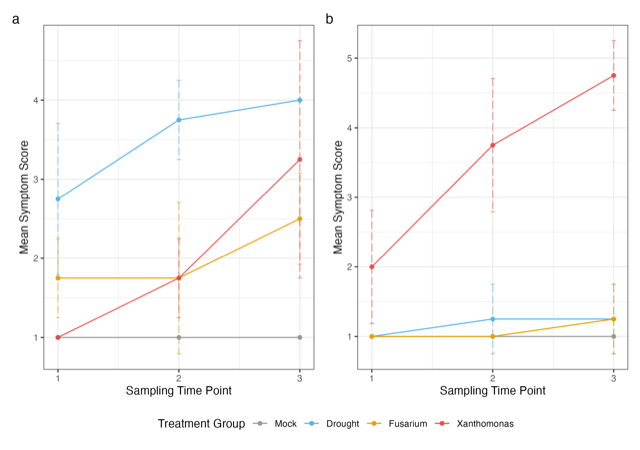
\includegraphics[width=\textwidth]{Figures/Combined_Sympotoms_plot.png}
    \caption[Symptom development scores of 'Grand Naine' plants infected with \acl{Focub4} or \acl{xvm}, or subjected to drought stress.]{\textbf{Symptom development scores of 'Grand Naine' plants infected with \acf{Focub4} or \acf{xvm}, or subjected to drought stress.} \textbf{a}) External symptom development. Symptoms were visually assessed based on chlorotic/wilting foliage, scored on a scale of 1–4: 1 = 0-25\%, 2 = 25-50\%, 3 = 50-75\%, 4 = 75-100\% .\textbf{b}) Internal symptom development. Symptoms were scored longitudinally at the rhizome: 1 = No discolouration, 2 = ≤ 5\%, 3 = 5-30\%, 4 = 30-50\%, 5 = 50-90\%, 6 = ≥ 90\%. Symptom scoring method was adapted from \textcite{Garcia-Bastidas2019}. Error bars show standard deviation.}
    \label{fig:SymptomDev}
\end{figure}



\begin{figure}[ph!]
    \centering
    \begin{subfigure}[b]{\textwidth}
        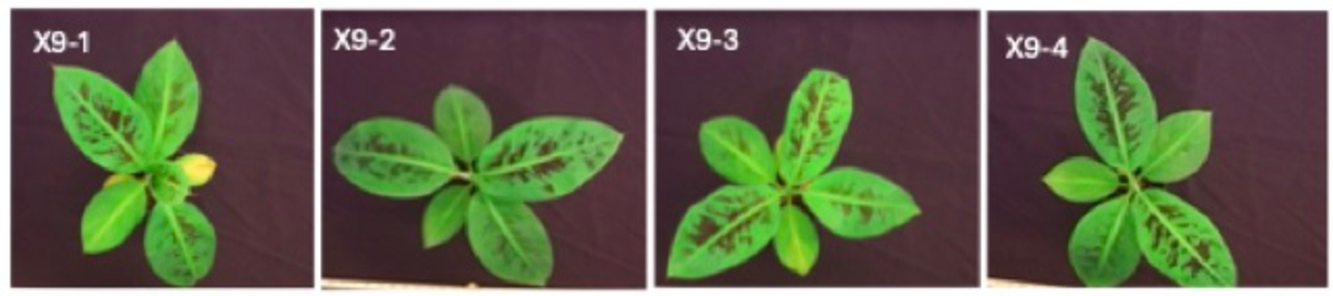
\includegraphics[width=\textwidth]{Figures/FirstTimePointXanthomonasBLQs.pdf}
        \caption{}
        \label{fig:XvmFirstTimeBLQs}
    \end{subfigure}
     \begin{subfigure}[b]{\textwidth}
        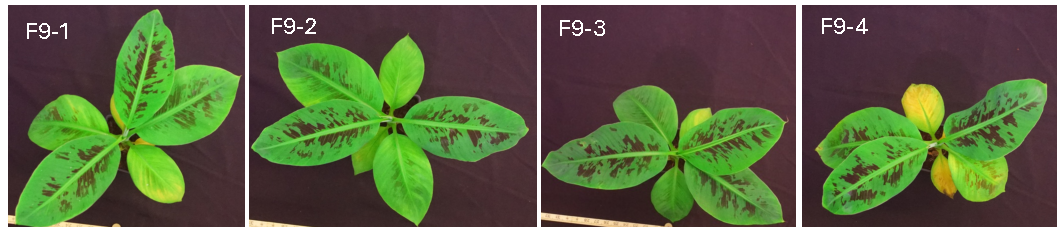
\includegraphics[width=\textwidth]{Figures/FirstTimePointFusariumBLQs.pdf}
        \caption{}
        \label{fig:FocFirstTimeBLQs}
    \end{subfigure}
         \begin{subfigure}[b]{\textwidth}
        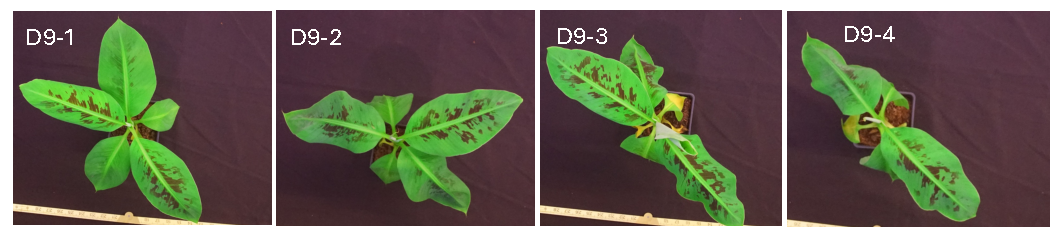
\includegraphics[width=\textwidth]{Figures/FirstTimePointDroughtBLQs.pdf}
        \caption{}
        \label{fig:DroFirstTimeBLQs}
    \end{subfigure}
         \begin{subfigure}[b]{\textwidth}
        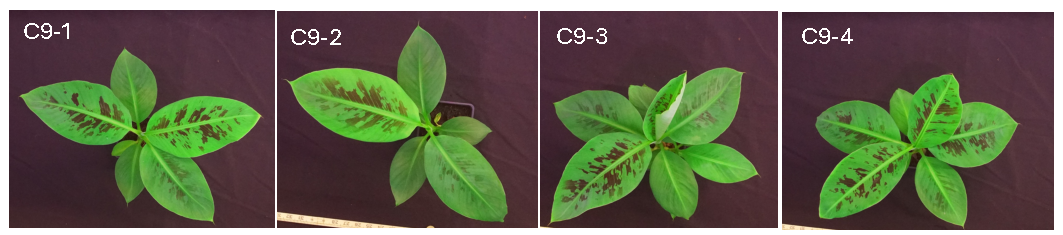
\includegraphics[width=\textwidth]{Figures/FirstTimePointControlBLQs.pdf}
        \caption{}
        \label{fig:ConFirstTimeBLQs}
    \end{subfigure}
    \caption[RGB images of 'Grande Naine' banana plants at the first sample time points.]{\textbf{RGB images of 'Grande Naine' banana plants at the first sample time points.}
    \textbf{\subref{fig:XvmFirstTimeBLQs}}) \acl{xvm}-inoculated plants at 7 \acl{dpi}.
    \textbf{\subref{fig:FocFirstTimeBLQs}}) \acl{Focub4}-inoculated plants at 15 \acl{dpi}.
    \textbf{\subref{fig:DroFirstTimeBLQs}}) Drought-stressed plants at 7 \ac{dpi}, no-watering.
    \textbf{\subref{fig:ConFirstTimeBLQs}}) Mock-inoculated plants at 7 \ac{dpi}.
    Plant labels are provided in white text and correspond to sample labels used in \acl{um} analysis.
    }
    \label{fig:FirstTimePointSymptoms}
\end{figure}

\begin{figure}[ph!]
    \centering
    \begin{subfigure}[b]{\textwidth}
        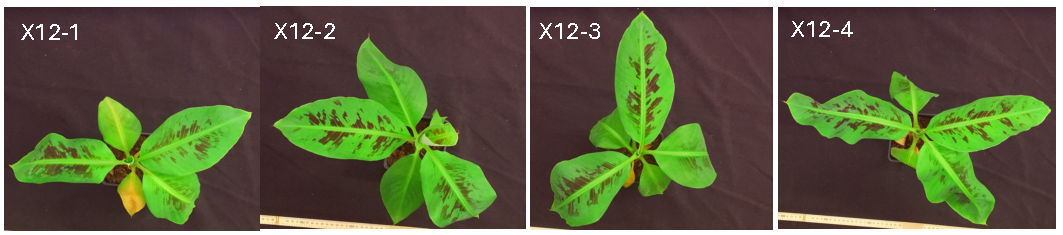
\includegraphics[width=\textwidth]{Figures/SecondTimePointXanthomonasBLQs.pdf}
        \caption{}
        \label{fig:XvmSecondTimeBLQs}
    \end{subfigure}
     \begin{subfigure}[b]{\textwidth}
        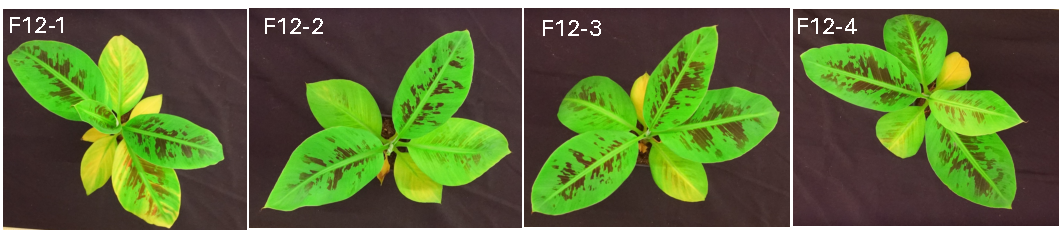
\includegraphics[width=\textwidth]{Figures/SecondTimePointFusariumBLQs.pdf}
        \caption{}
        \label{fig:FocSecondTimeBLQs}
    \end{subfigure}
         \begin{subfigure}[b]{\textwidth}
        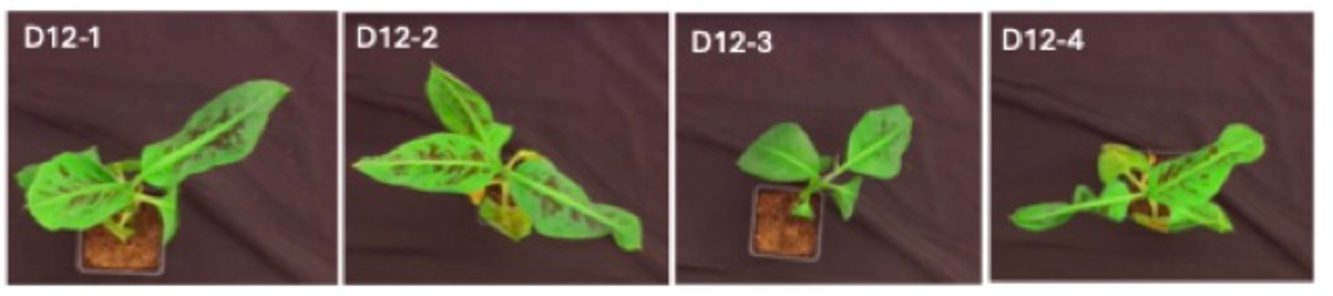
\includegraphics[width=\textwidth]{Figures/SecondTimePointDroughtBLQs.pdf}
        \caption{}
        \label{fig:DroSecondTimeBLQs}
    \end{subfigure}
         \begin{subfigure}[b]{\textwidth}
        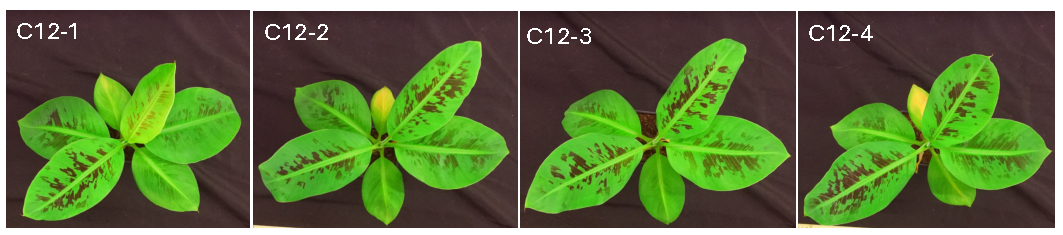
\includegraphics[width=\textwidth]{Figures/SecondTimePointControlBLQs.pdf}
        \caption{}
        \label{fig:ConSecondTimeBLQs}
    \end{subfigure}
    \caption[RGB images of 'Grande Naine' banana plants at the second sample time points.]{\textbf{RGB images of 'Grande Naine' banana plants at the second sample time points.}
    \textbf{\subref{fig:XvmSecondTimeBLQs}}) \acl{xvm}-inoculated plants at 10 \acl{dpi}.
    \textbf{\subref{fig:FocSecondTimeBLQs}}) \acl{Focub4}-inoculated plants at 18 \acl{dpi}.
    \textbf{\subref{fig:DroSecondTimeBLQs}}) Drought-stressed plants at 10, no-watering.
    \textbf{\subref{fig:ConSecondTimeBLQs}}) Mock-inoculated plants at 10 \ac{dpi}.
    Plant labels are provided in white text and correspond to sample labels used in \acl{um} analysis.
    }
    \label{fig:SecondTimePointSymptoms}
\end{figure}

\begin{figure}[ph!]
    \centering
    \begin{subfigure}[b]{\textwidth}
        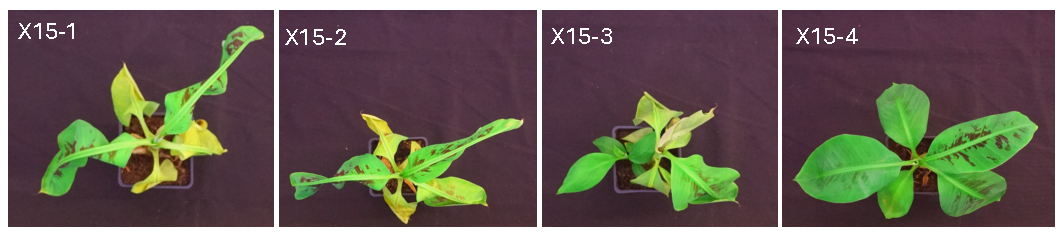
\includegraphics[width=\textwidth]{Figures/ThirdTimePointXanthomonasBLQs.pdf}
        \caption{}
        \label{fig:XvmThirdTimeBLQs}
    \end{subfigure}
     \begin{subfigure}[b]{\textwidth}
        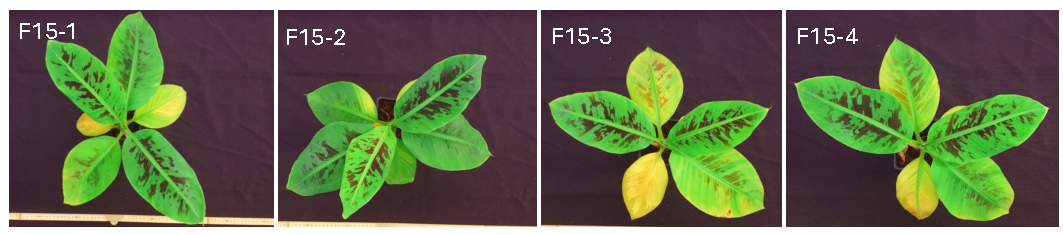
\includegraphics[width=\textwidth]{Figures/ThirdTimePointFusariumBLQs.pdf}
        \caption{}
        \label{fig:FocThirdTimeBLQs}
    \end{subfigure}
         \begin{subfigure}[b]{\textwidth}
        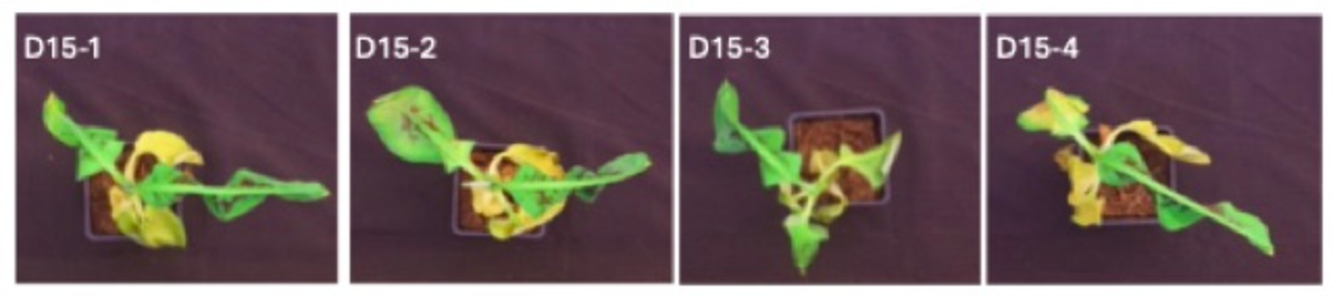
\includegraphics[width=\textwidth]{Figures/ThirdTimePointDroughtBLQs.pdf}
        \caption{}
        \label{fig:DroThirdTimeBLQs}
    \end{subfigure}
         \begin{subfigure}[b]{\textwidth}
        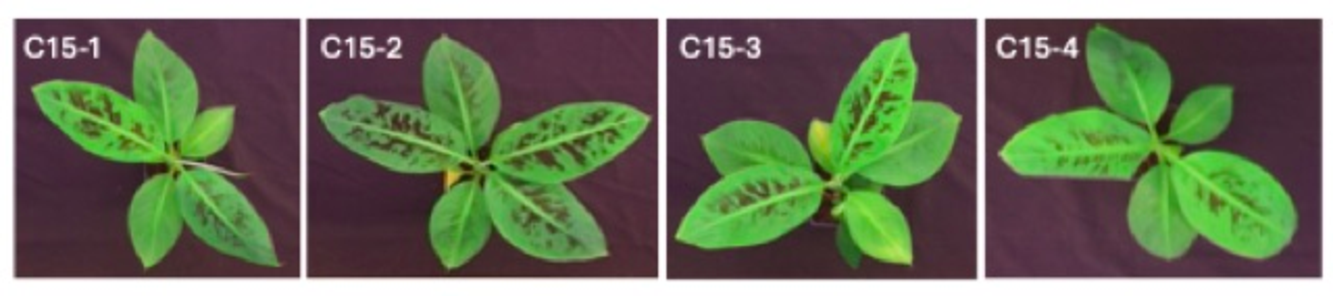
\includegraphics[width=\textwidth]{Figures/ThirdTimePointControlBLQs.pdf}
        \caption{}
        \label{fig:ConThirdTimeBLQs}
    \end{subfigure}
    \caption[RGB images of 'Grande Naine' banana plants at the third sample time points.]{\textbf{RGB images of 'Grande Naine' banana plants at the third sample time points.}
    \textbf{\subref{fig:XvmThirdTimeBLQs}}) \acl{xvm}-inoculated plants at 13 \acl{dpi}.
    \textbf{\subref{fig:FocThirdTimeBLQs}}) \acl{Focub4}-inoculated plants at 21 \acl{dpi}.
    \textbf{\subref{fig:DroThirdTimeBLQs}}) Drought-stressed plants at 13, no-watering.
    \textbf{\subref{fig:ConThirdTimeBLQs}}) Mock-inoculated plants at 13 \ac{dpi}.
    Plant labels are provided in white text and correspond to sample labels used in \acl{um} analysis.
    }
    \label{fig:ThridTimePointSymptoms}
\end{figure}

\subsection{Metabolite profiling and clustering analysis in response to wilting stresses}

To identify metabolites that can distinguish the wilting stresses, three lamina samples from each plant were collected and homogenised. Metabolites were extracted and \ac{lcms} with \ac{esi} was performed. Samples were processed using the two polarity modes available, positive ion mode, which charges analytes through protonation, and negative ion mode, which charges analytes through deprotonation. Positive and negative mode data were analysed separately. 

Using the positive mode data, a total of 2,294 aligned features\footnote{In \ac{lcms}, eluting compounds generate multiple mass signals, including adducts, fragments, and isotopic peaks, resulting in several two-dimensional features. Therefore, we use the term 'feature' to refer to these bounded, two-dimensional signals characterised by the mass-to-charge ratio ($m/z$) and retention time, aligning with the terminology used by Tautenhahn et al. (2008).} were detected across all samples, divided into groups by treatment and time point, using XCMSOnline (v2.7.2) \parencite{Gowda2014} (following the retention time and CAMERA annotated adduct filtering). Of the 2,294 aligned features, 633 were identified as statistically significant ($p \le0.05$) by a one-way \ac{anova}. Hierarchical clustering of samples and the 633 significant features ($p \le0.05$) revealed that sample groups clustered by time, except \ac{xvm}-inoculated samples from the first time point (7 \ac{dpi}) (Figure \ref{fig:Sig657FeaturesRedSamples}). Samples from the same treatment group did not all cluster together when using the 633 significant features ($p \le0.05$).

Similarly, 2,180 aligned features were identified using the negative mode data, where samples were divided into groups by treatment and time point (following the retention time and CAMERA annotated adduct filtering). A one-way \ac{anova} of 
the aligned features from the negative mode data identified 453 significant features ($p \le0.05$). Hierarchical clustering of samples and the 453 significant features revealed that, unlike the features identified from the positive mode data, samples did not form an obvious general clustering pattern (Appendix C\ref{apx:}). 
 
\begin{figure}[hp!]
    \centering
    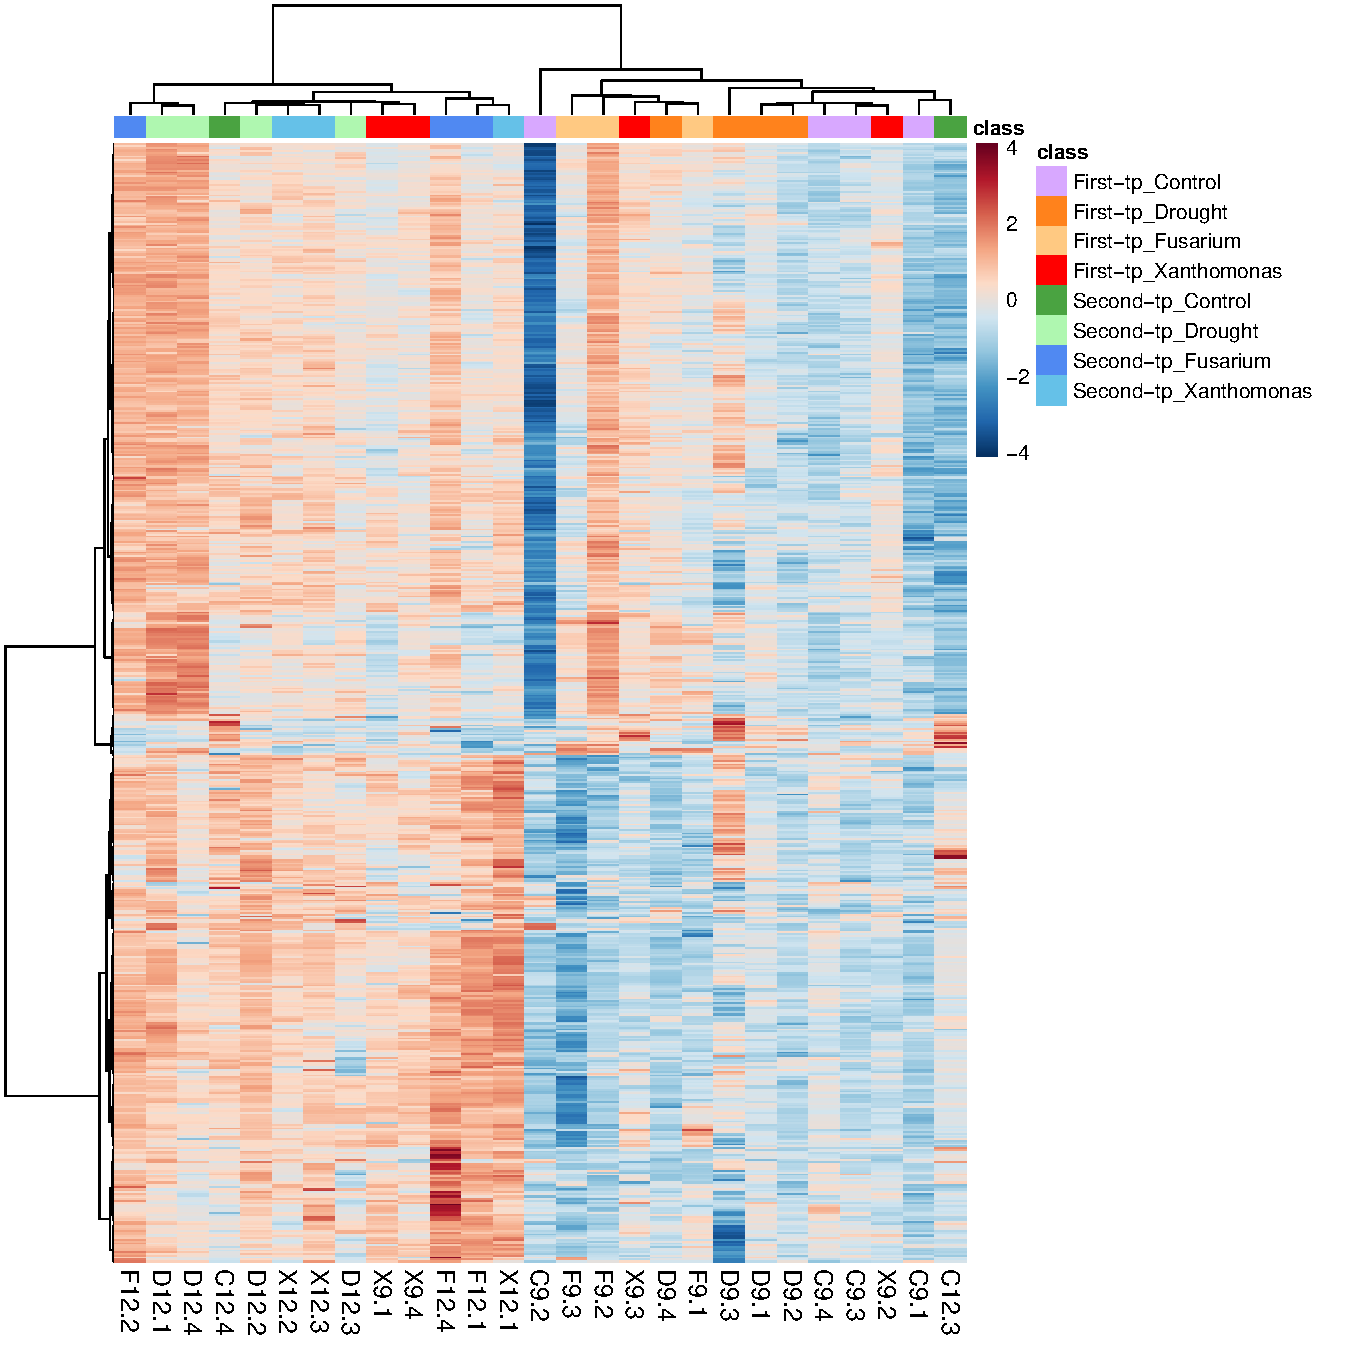
\includegraphics[width=\textwidth]{Figures/Sig633FeaturesRedSamplesRedGroups_ForThesis.pdf}
    \caption[Heatmap showing hierarchical clustering of samples based on 633 normalised significant feature peak intensities ($p \le0.05$).]{\textbf{Heatmap showing hierarchical clustering of samples based on 633 normalised significant feature peak intensities ($p \le0.05$).}The distance measure was Euclidean and the ward.D algorithm was used for clustering. Class shows the treatment and time groups. Value shows the normalised peak intensity. Features were normalised to the sodium formate Na(NaCOOH)3 adduct ($m/z=226.9521$), log-transformed and scaled (Pareto scaling). tp =  time point. Mock-inoculated samples are labelled as "Control". Figure generated using MetaboAnalyst (v6.0).}
    \label{fig:Sig657FeaturesRedSamples}
\end{figure}


To identify treatment-specific characteristics rather than temporal variations, we separated samples into discrete time points for subsequent analysis. Of the 2,294 aligned features from the positive mode data, 232 were identified as significant ($p \le0.05$) using a one-way \ac{anova} at the first time point. When hierarchical clustering was performed using these 232 significant features ($p \le0.05$), samples from the first time point mostly clustered into their respective treatment groups (Figure \ref{fig:Sig232FeaturesRedSamples}). One sample from the drought-stressed treatment, D9.4, clustered with the \ac{Focub4}-inoculated samples from the first time point. Additionally, sample C9.2, from the mock-inoculated treatment, did not cluster with the mock-inoculated group (Figure \ref{fig:Sig232FeaturesRedSamples}). C9.2 recorded lower peak intensities for many of the significant features when compared to the other mock-inoculated samples (Figure \ref{fig:Sig232FeaturesRedSamples}). This analysis was repeated with the negative mode data, which identified 56 significant features ($p \le0.05$) \textcolor{red}{(ADD FIGURE TO APPENDIX)}. Mock-inoculated samples clustered separately when hierarchical clustering was performed on samples using the negative mode dataset, however, samples from the treatments did not form distinct groups \textcolor{red}{(ADD FIGURE TO APPENDIX)}.


\begin{figure}[hp!]
    \centering
    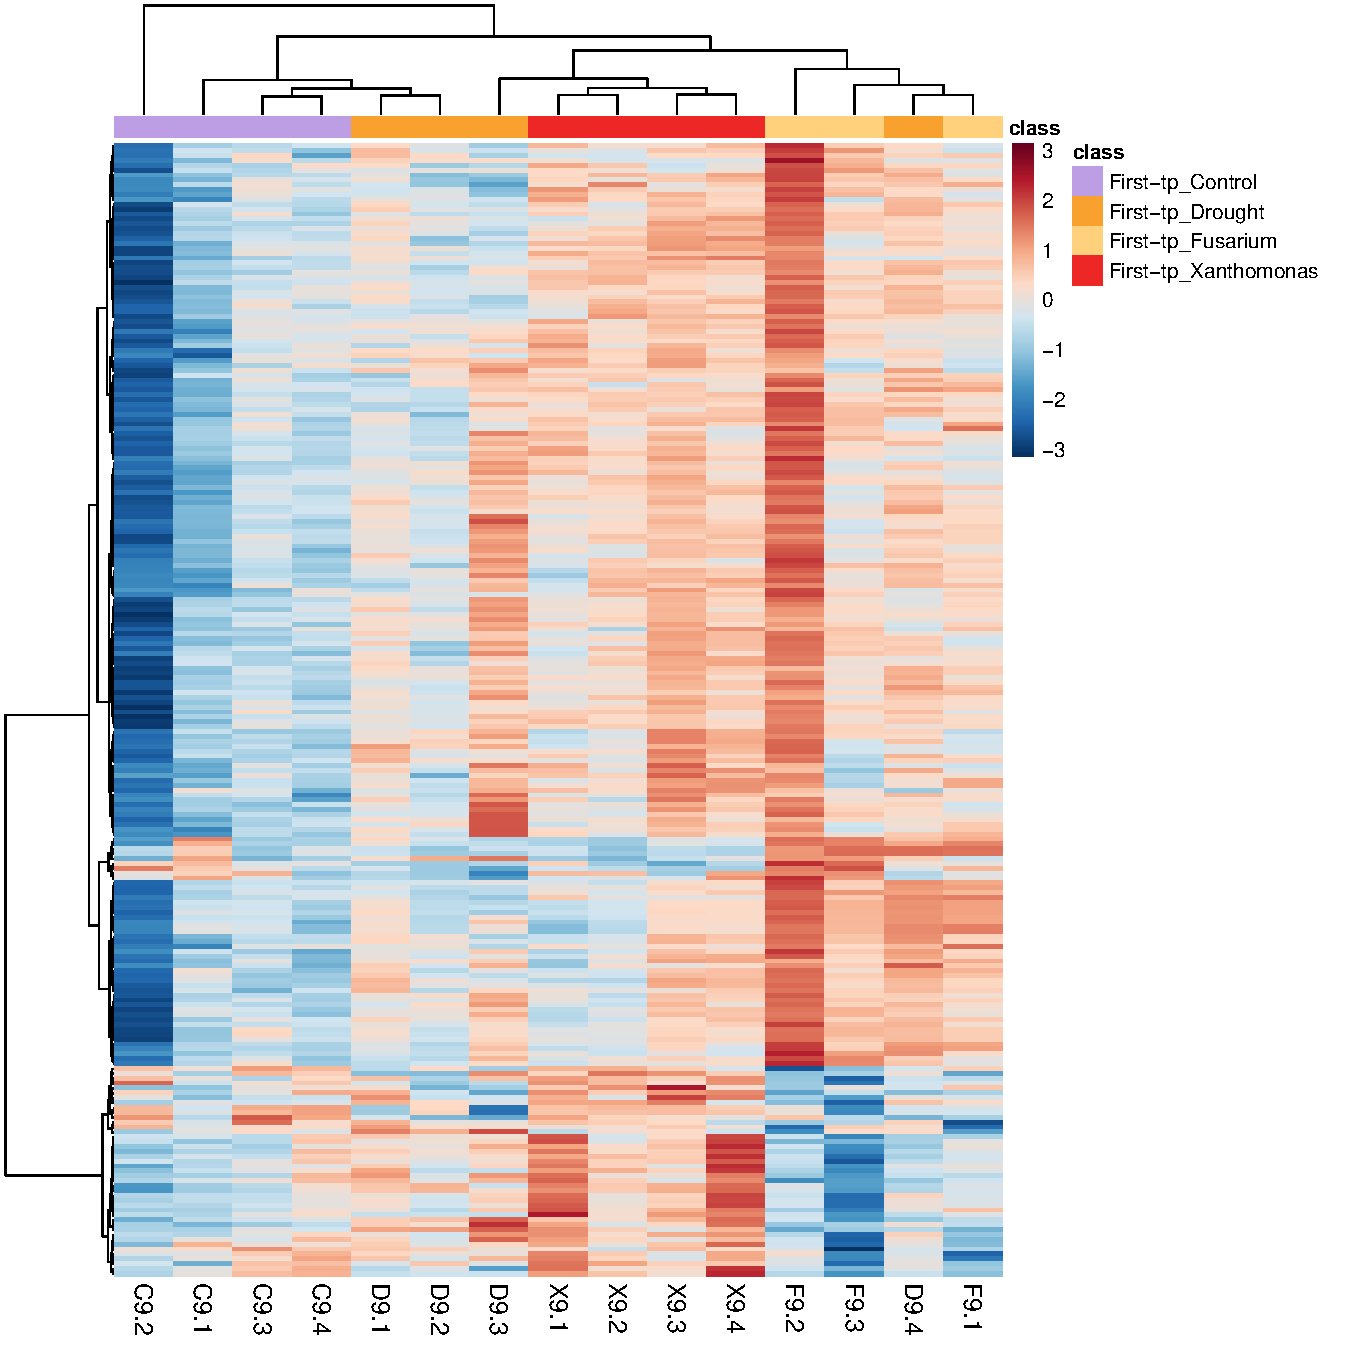
\includegraphics[width=\textwidth]{Figures/Sig232Features_heatmap_9_dpi72-ForThesis.pdf}
    \caption[Heatmap showing hierarchical clustering of samples based on 232 normalised significant feature peak intensities ($p \le0.05$) from the first time point (positive mode).]{\textbf{Heatmap showing hierarchical clustering of samples based on 232 normalised significant feature peak intensities ($p \le0.05$) from the first time point (positive mode).} The distance measure was Euclidean and the ward.D algorithm was used for clustering. Class shows the treatment and time groups. Value shows the normalised peak intensity. Features were normalised to the sodium formate Na(NaCOOH)3 adduct ($m/z=226.9521$), log-transformed and scaled (Pareto scaling). tp =  time point. Mock-inoculated samples are labelled as "Control".  Figure generated using MetaboAnalyst (v6.0).}
    \label{fig:Sig232FeaturesRedSamples}
\end{figure}

At the second time point, only 171 significant features ($p \le0.05$) were identified (unequal group variance) from the positive mode data. When hierarchical clustering was performed on these features, samples clustered based on the treatment group (Figure \ref{fig:Sig171FeaturesRedSamples}). However, one sample from the drought-stress treatment, D12.2, clustered with the samples from the \ac{xvm}-inoculated group. \Ac{plsda} of the 171 features from the second time point revealed clear discrimination of the \ac{Focub4}-inoculated, \ac{xvm}-inoculated, drought-stressed, and mock-inoculated plants based on their feature profiles (Figure \ref{fig:FeaturesTimePoint_plsda}). 

We also identified significant features from the negative mode data at the second time point. As the data did not follow a normal distribution, a non-parametric \ac{anova} was performed, revealing 806 significant features ($p\le0.05$). Hierarchical clustering was performed using these 806 features and, unlike the positive mode data, all samples grouped by treatment \textcolor{red}{(APPENDIX FIGURE)}. 

\label{section:T1AndT2Adducts}
To find viable biomarkers, metabolites must distinguish wilting stresses over time. Therefore, we compared the significant features identified at the first and second-time points (232 and 171, respectively) from the positive mode data. Only six significant features were shared (Figure \ref{fig:FeaturesTimePoint_Venn}). As a total of six shared features is low, we checked for potentially shared metabolites by identifying features with the same retention times ($\le1$ second), and $m/z$ values that differ by the nominal masses of common \ac{lcms} adducts, (e.g. [M+H]\textsuperscript{+}, [M+Na]\textsuperscript{+}, [M+K]\textsuperscript{+}). This identified a further set of 19 potentially shared metabolites. 

\begin{figure}[!hptb]
    \centering
    \begin{subfigure}[b]{0.42\textwidth}
        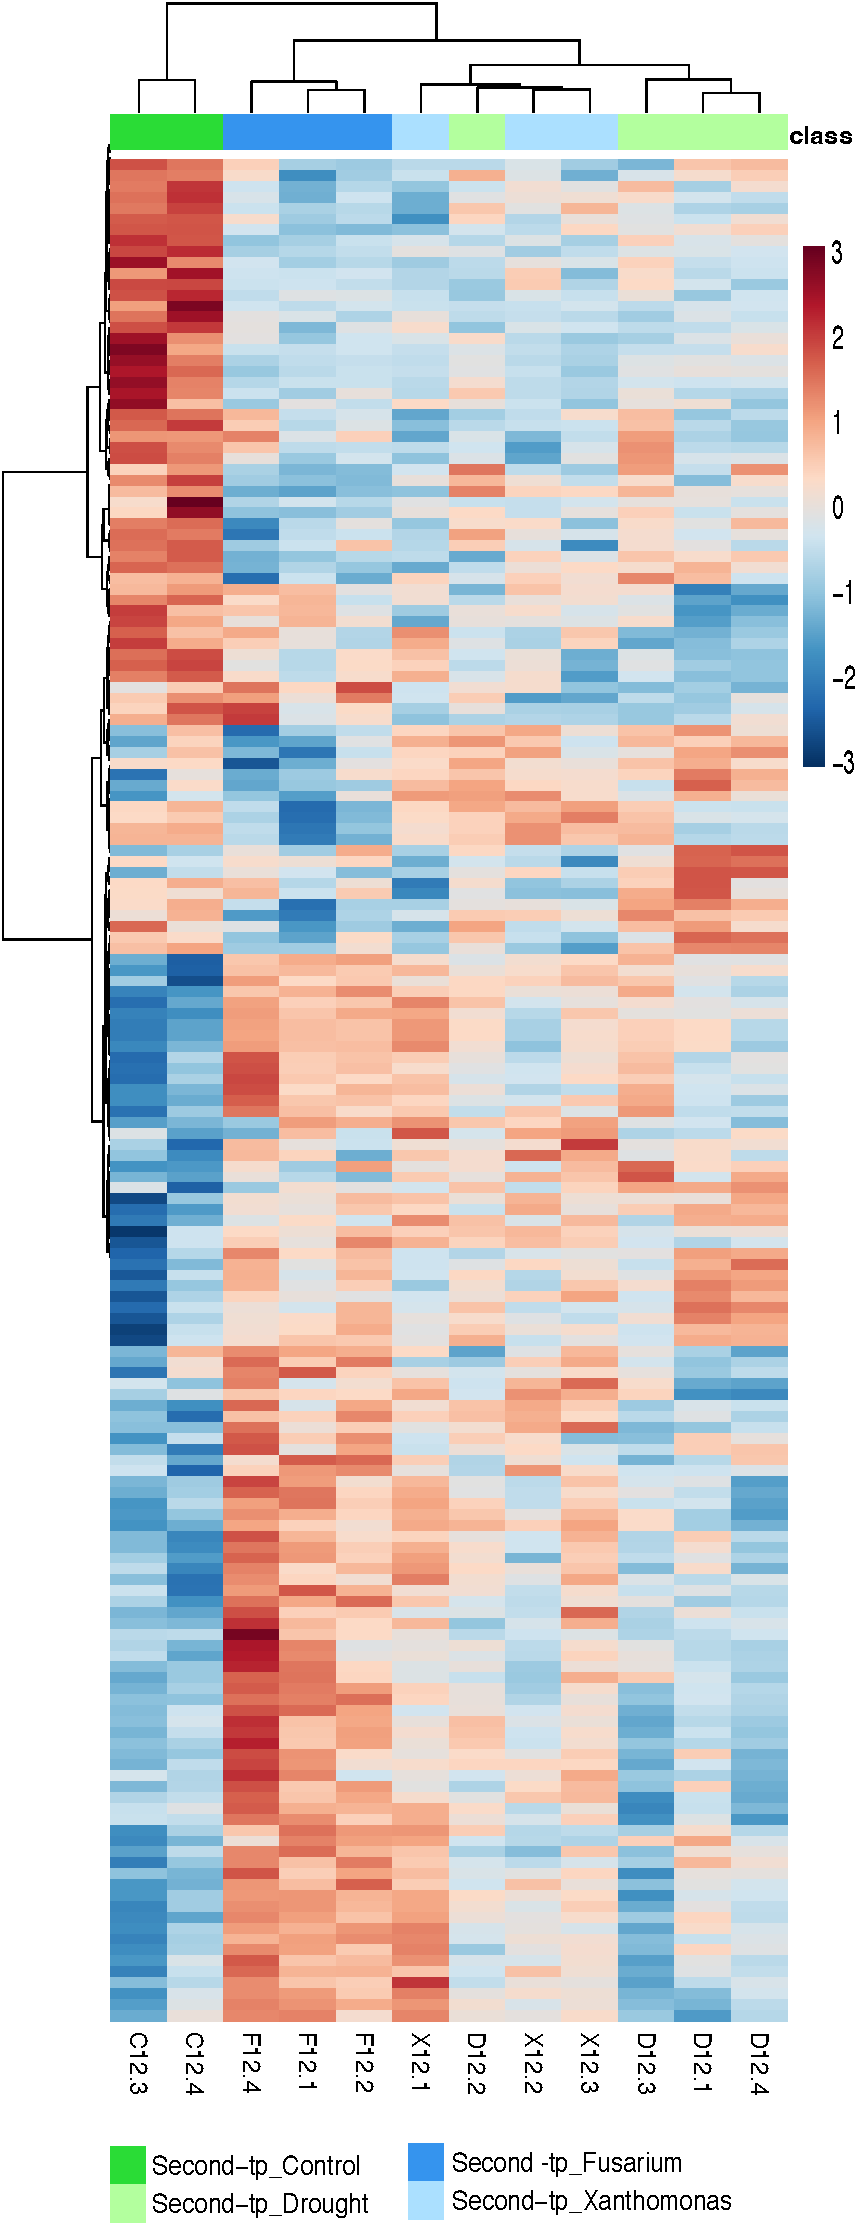
\includegraphics[width=\textwidth]{Figures/heatmapofsigfeatures-ForThesis-Long.pdf}
      \caption{}
      \label{fig:Sig171FeaturesRedSamples}
    \end{subfigure}
    \hfill
    \begin{minipage}[b]{0.57\textwidth}
      \begin{subfigure}[b]{\linewidth}
      \begin{subfigure}[b]{\linewidth}
	    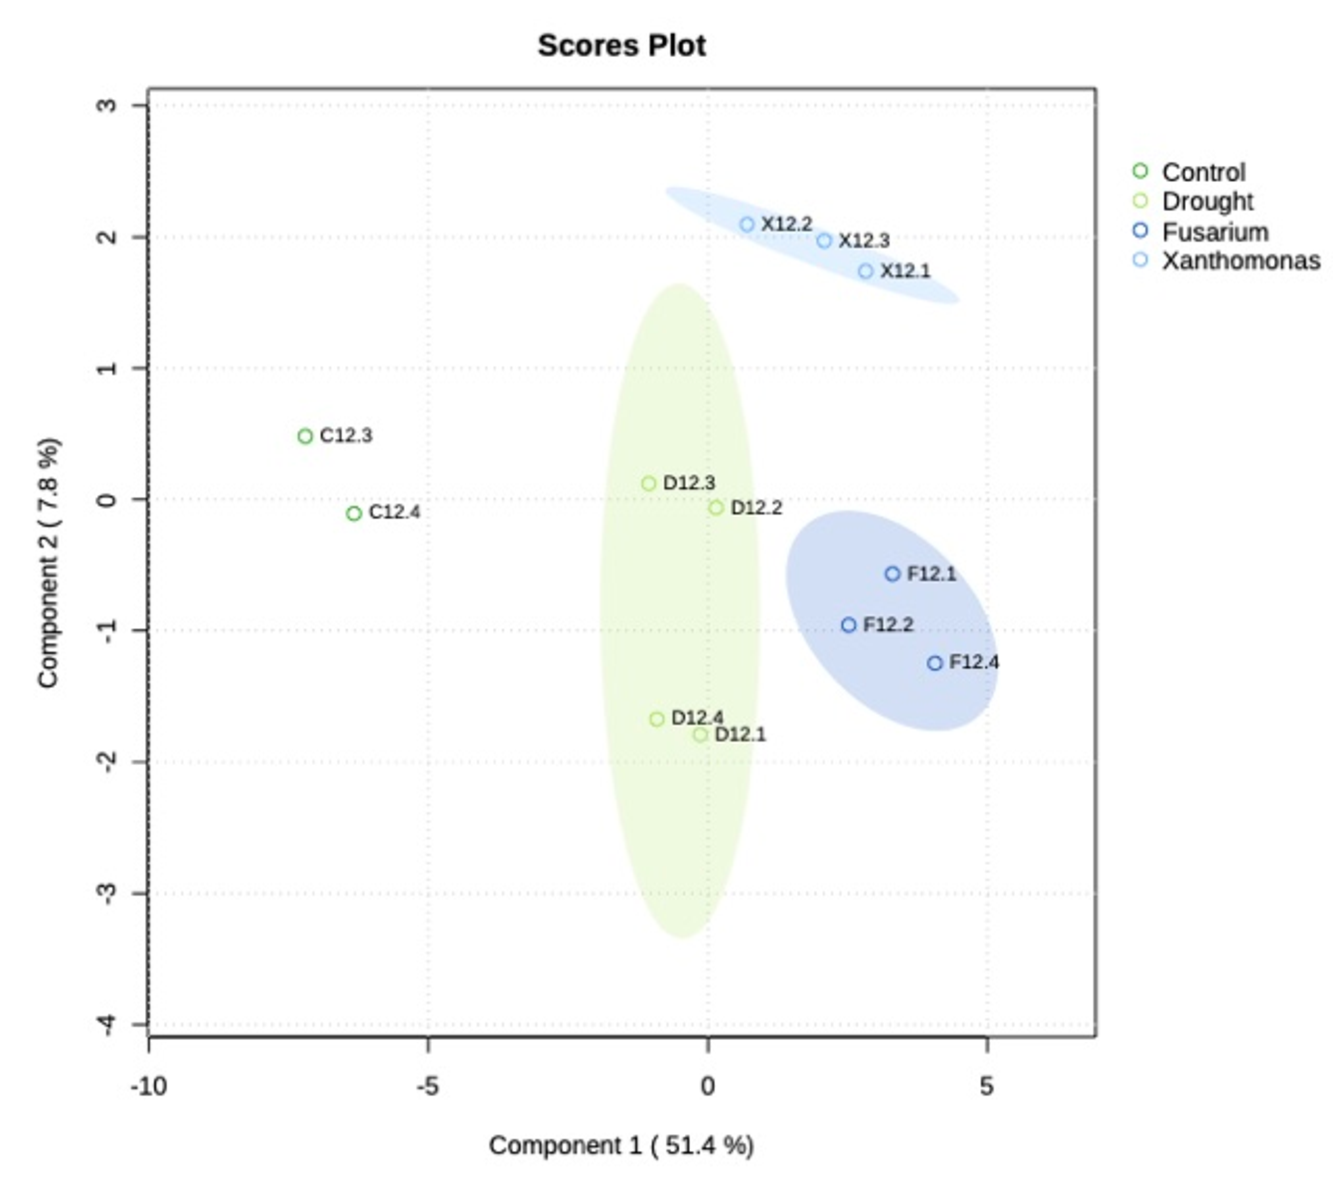
\includegraphics[width=\textwidth]{Figures/PLSDA_SigFeaturesRedSamplesRedGroupsSecondTimePoint.pdf}
        \caption{}
        \label{fig:FeaturesTimePoint_plsda}
      \end{subfigure}
	    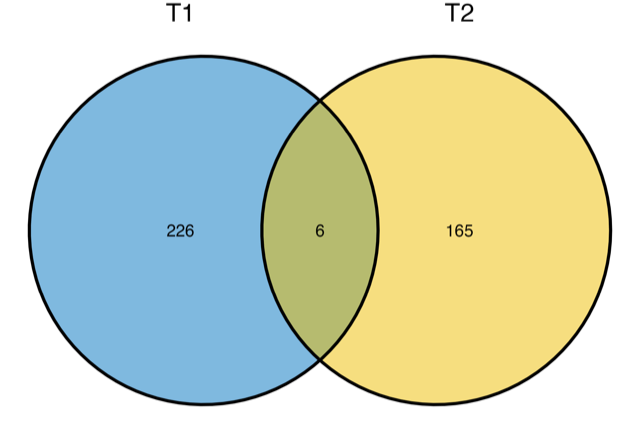
\includegraphics[width=\textwidth]{Figures/SharedFeaturesVenn_Time.png}
        \caption{}
        \label{fig:FeaturesTimePoint_Venn}
      \end{subfigure}\\[\baselineskip]
    \end{minipage}
    \caption[Distribution of features at the second time point (positive mode).]{\textbf{Distribution of significant features at the second time point (positive mode).}
    \textbf{\subref{fig:Sig171FeaturesRedSamples}}) Heatmap showing hierarchical clustering of samples based on 171 normalised significant feature peak intensities ($p \le0.05$). The distance measure was Euclidean and the ward.D algorithm was used for clustering. Class shows the treatment and time groups. Value shows the normalised peak intensity. Features were normalised to the sodium formate Na(NaCOOH)3 adduct ($m/z=226.9521$), log-transformed and scaled (Pareto scaling). 
    \textbf{\subref{fig:FeaturesTimePoint_plsda}}) \acl{plsda} score plot of significant features at the second time point. 
    \textbf{\subref{fig:FeaturesTimePoint_Venn}}) Shared significant features ($p \le0.05$) between the first two time points. T1 = first-time point, T2 = second-time point.
    Figures \subref{fig:Sig171FeaturesRedSamples} and \subref{fig:FeaturesTimePoint_plsda} were generated using MetaboAnalyst (v6.0). 
    }
    \label{fig:SecondTimePointSigFig}
\end{figure}

\subsection{Specific discriminant features from each treatment group }

To identify features capable of discriminating different wilt-stressed and mock-inoculated plants, pairwise analyses were conducted using the abundances of the 171 significant features from the second time point positive mode data. Though two mock-inoculated samples is too low a sample number to conclude a meaningful difference, we used  Students' t-tests (unequal group variance) to identify features of interest. When comparing \ac{Focub4}-inoculated plants to mock-inoculated plants, we identified 63 features of interest (Figure  \ref{fig:FocVsCon_t-test}). In the \ac{xvm}-inoculated to mock-inoculated pairwise comparison, 48 features of interest were identified. Similarly, 48 features of interest were identified in the drought-stressed to mock-inoculated pairwise comparison (Figure  \ref{fig:XvmVsCon_t-test} and \ref{fig:DroVsCon_t-test}). We searched for exact matches of the features of interest (n=159) between the wilt-stress treatments and identified 25 that were shared between all treatments, 18 that were potentially unique to \ac{Focub4}-inoculated, eight that were potentially unique to \ac{xvm}-inoculated, and six that were potentially unique to drought-stressed plants (Figure  \ref{fig:PairwiseVenn-SecondTimePoint}).

To establish reliable biomarkers, target metabolites need to be consistently present across multiple sampling points. Consequently, we compared the potentially unique sets of features with those shared between the first and second time points (see \ref{section:T1AndT2Adducts}). Features that were absent at either the first or second time point, or those containing differences in mass ($m/z$) that correspond to common losses (e.g. hexose, 162Da; glucose, 180Da; water 18Da), potential adducts or contaminants identified as features of interest in other treatment groups, were excluded from the analysis.

\begin{figure}[hp!]
    \centering
    \begin{subfigure}[b]{0.49\textwidth}
        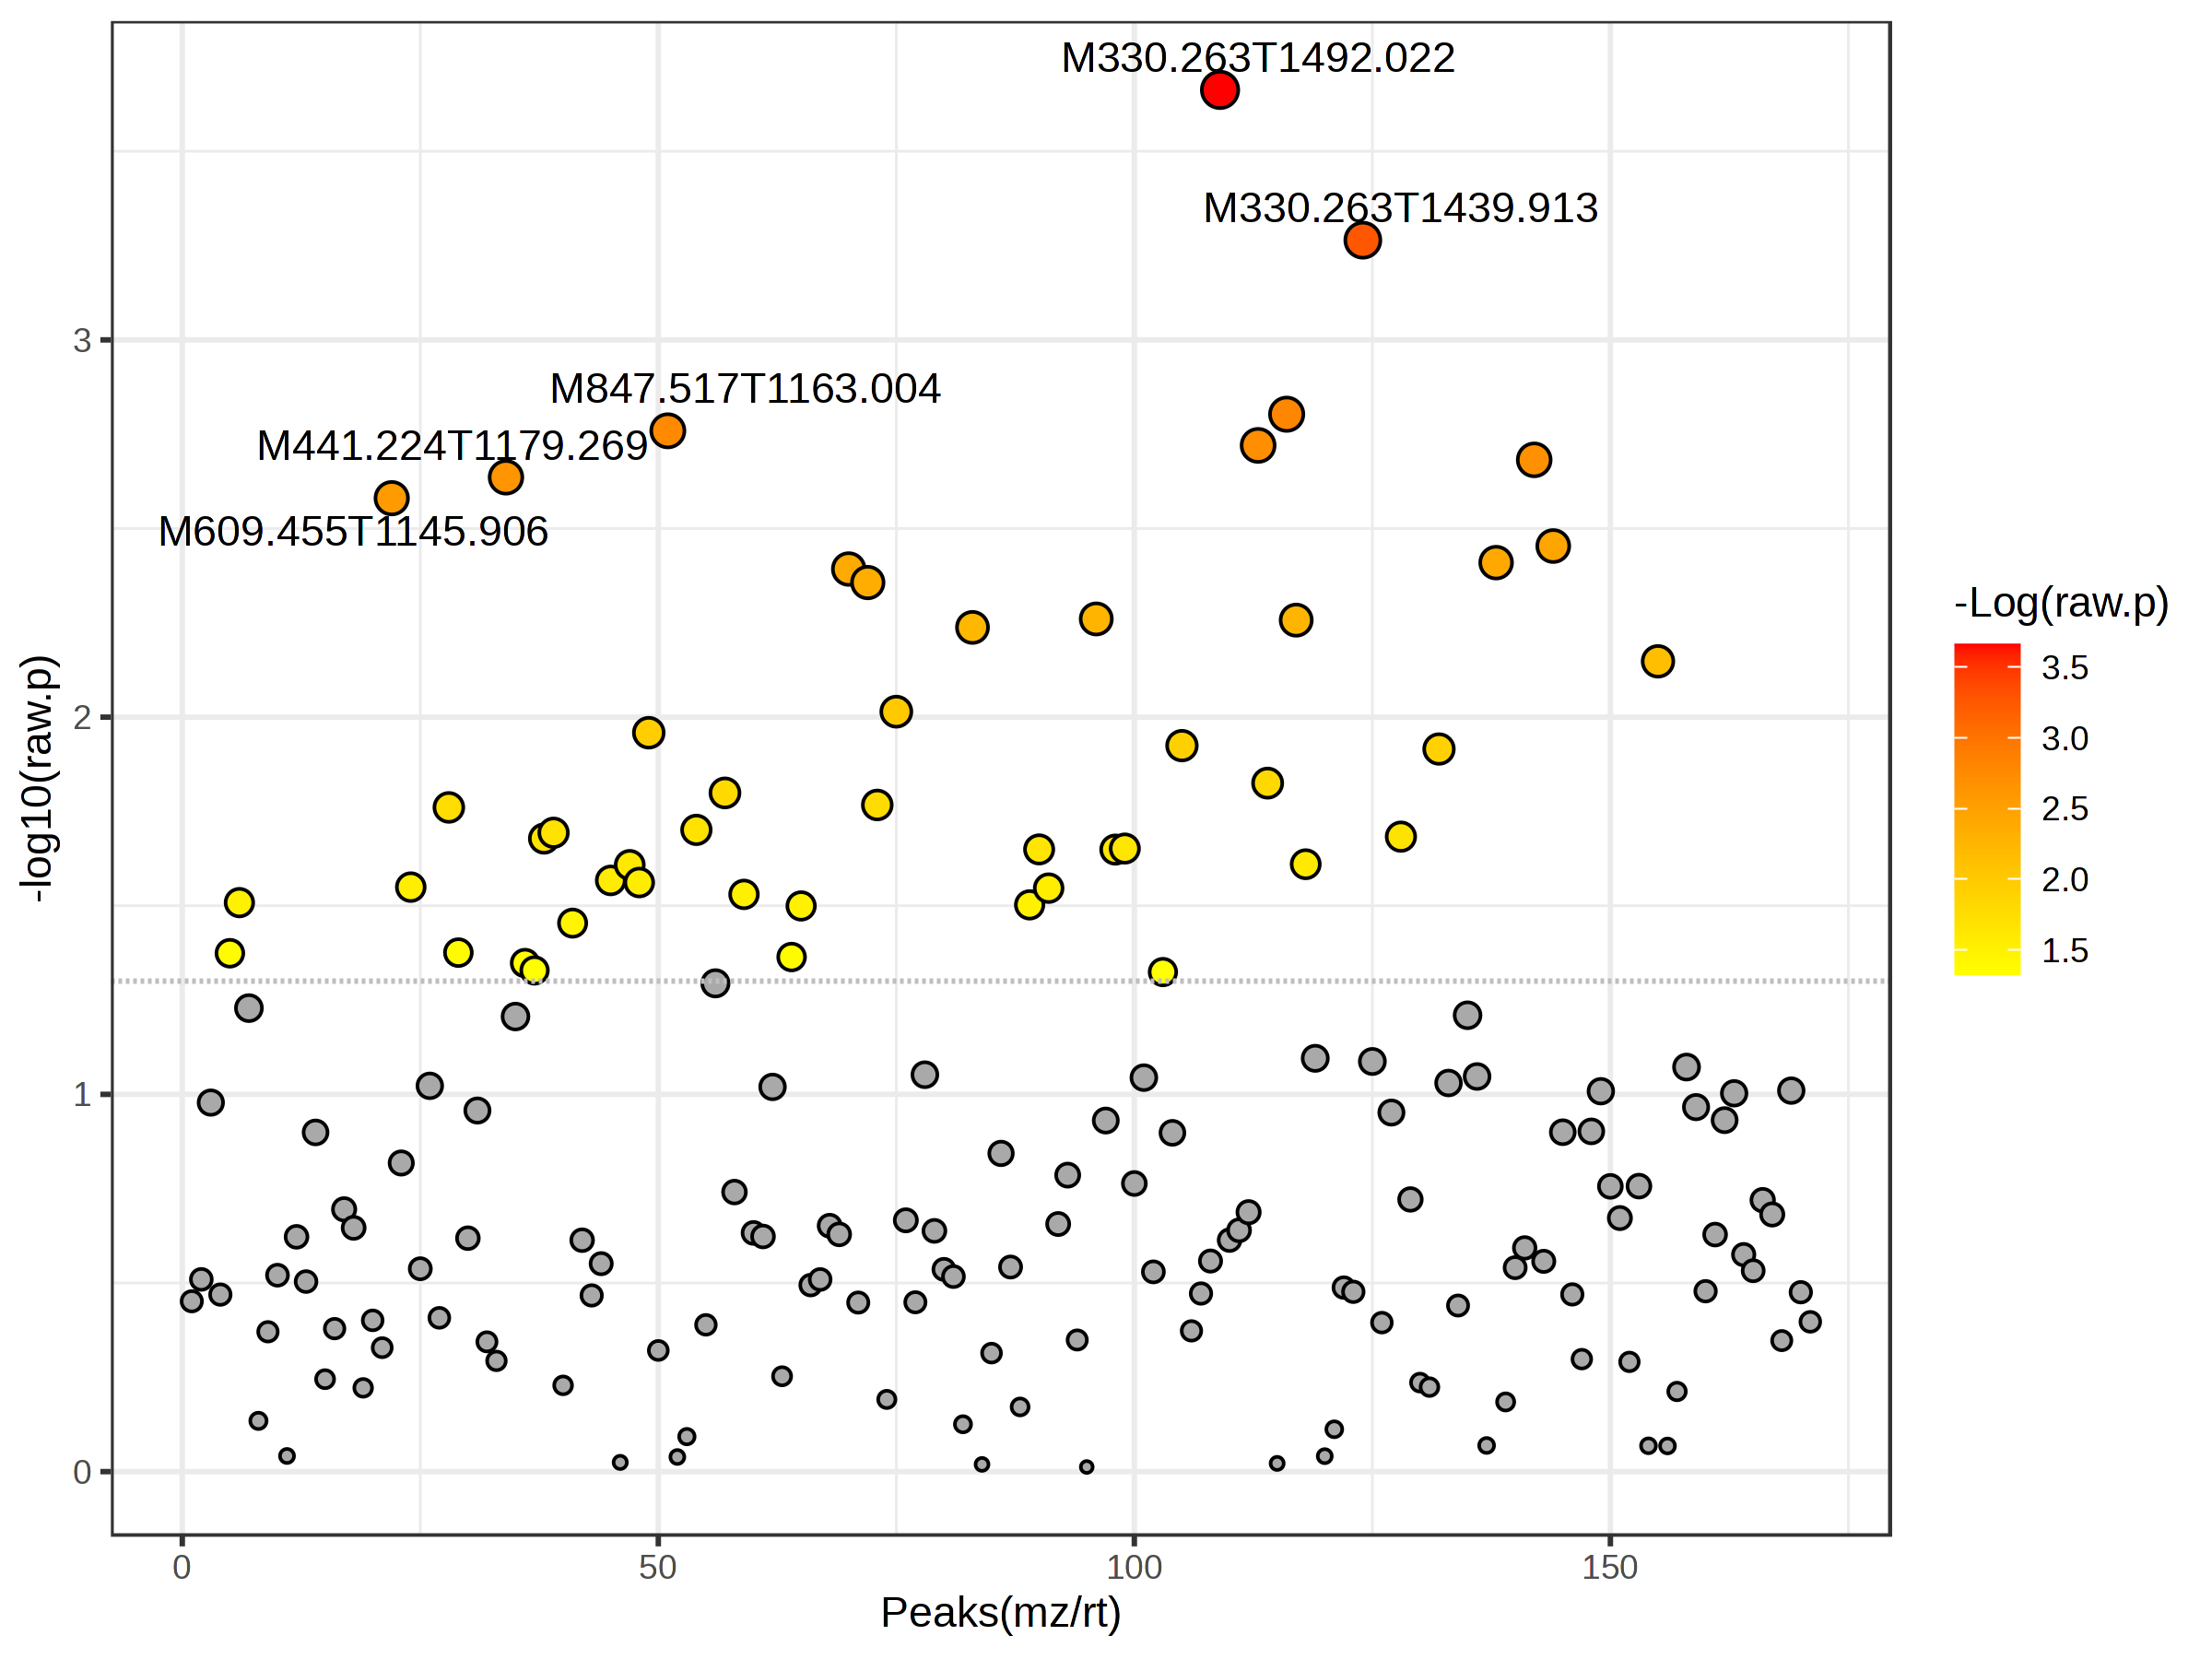
\includegraphics[width=\textwidth]{Figures/Sig171FeaturesRedGroupsDroVsConSecondTimePoint_t-test.png}
        \caption{}
        \label{fig:DroVsCon_t-test}
    \end{subfigure}
    \begin{subfigure}[b]{0.49\textwidth}
        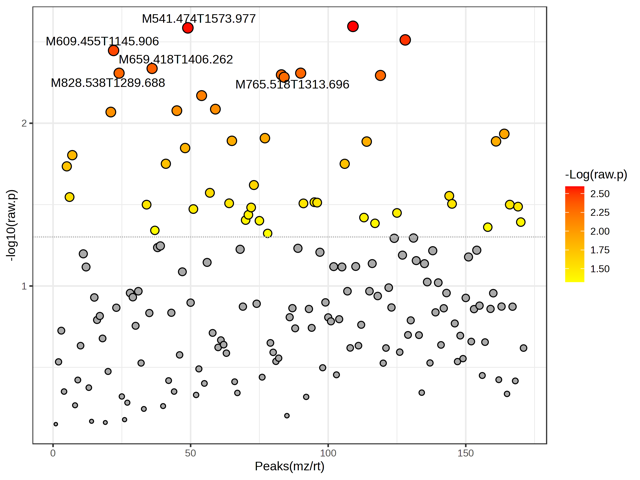
\includegraphics[width=\textwidth]{Figures/Sig171FeaturesRedSamplesXvmVsConSecondTimePoint_t_test.png}
        \caption{}
        \label{fig:XvmVsCon_t-test}
    \end{subfigure}
    \begin{subfigure}[b]{0.49\textwidth}
        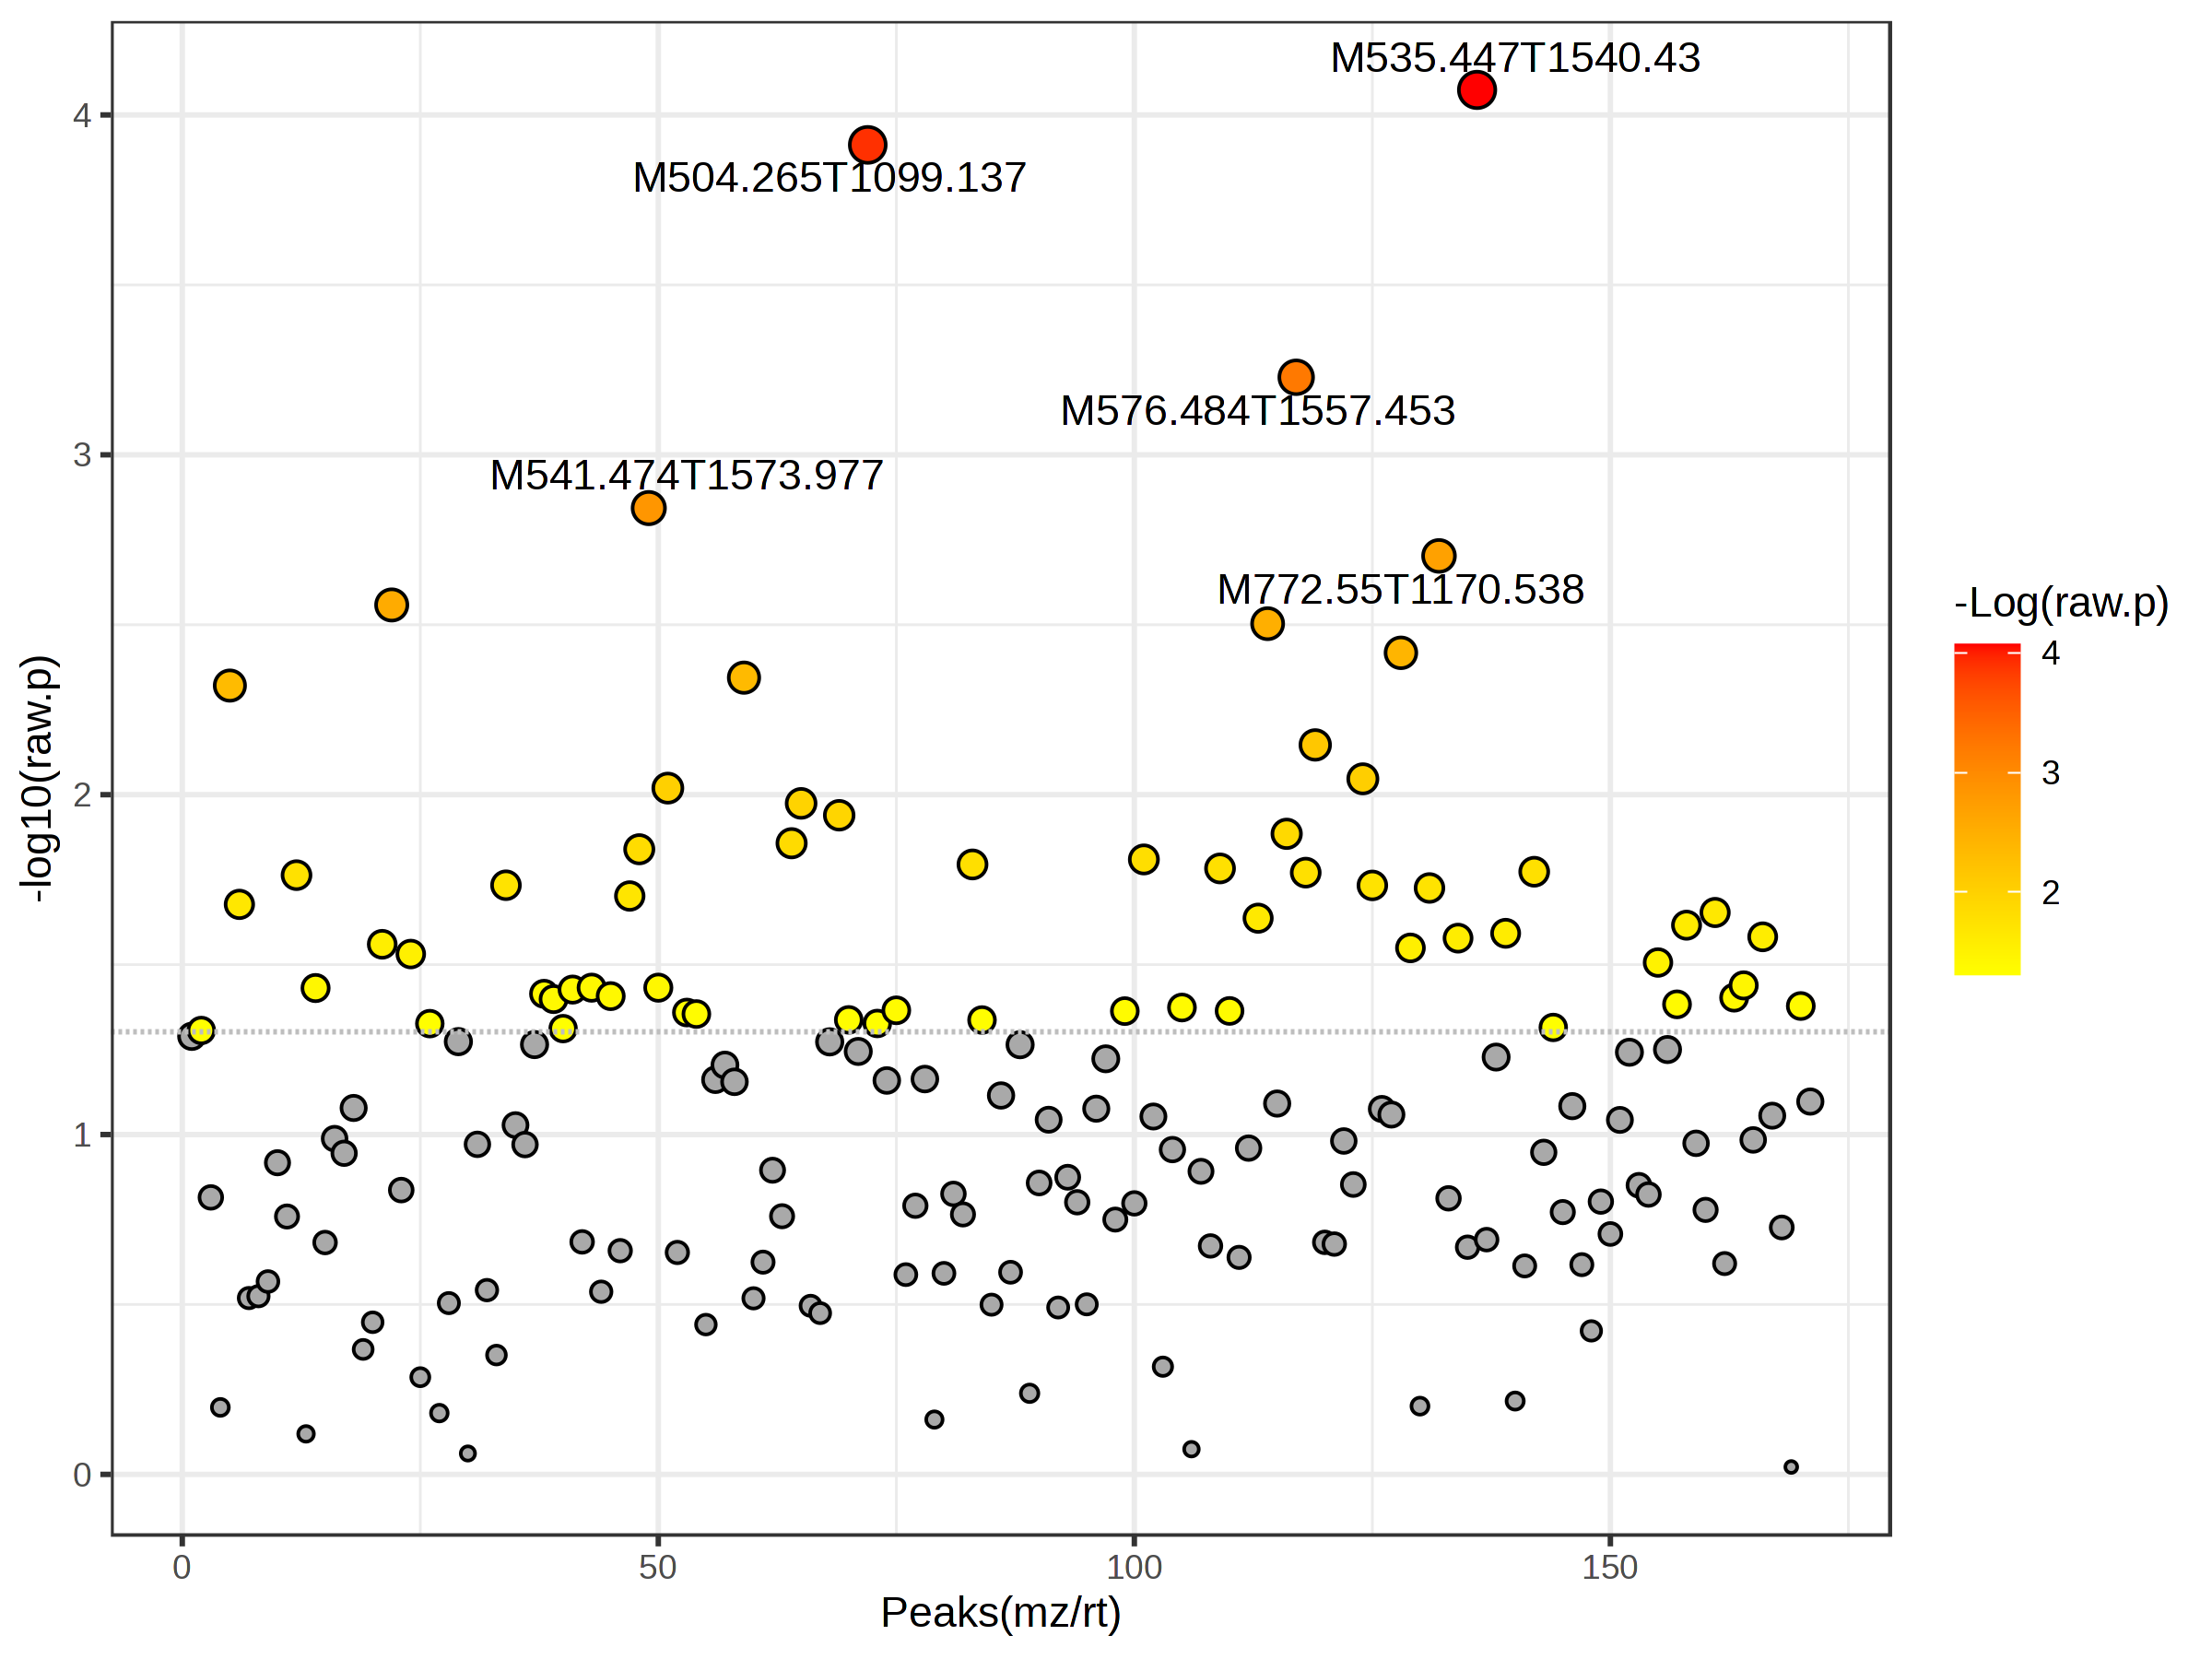
\includegraphics[width=\textwidth]{Figures/Sig171FeaturesRedSamplesFocVsConSecondTimePoint_t_test.png}
        \caption{}
        \label{fig:FocVsCon_t-test}
    \end{subfigure}
    \begin{subfigure}[b]{0.47\textwidth}
        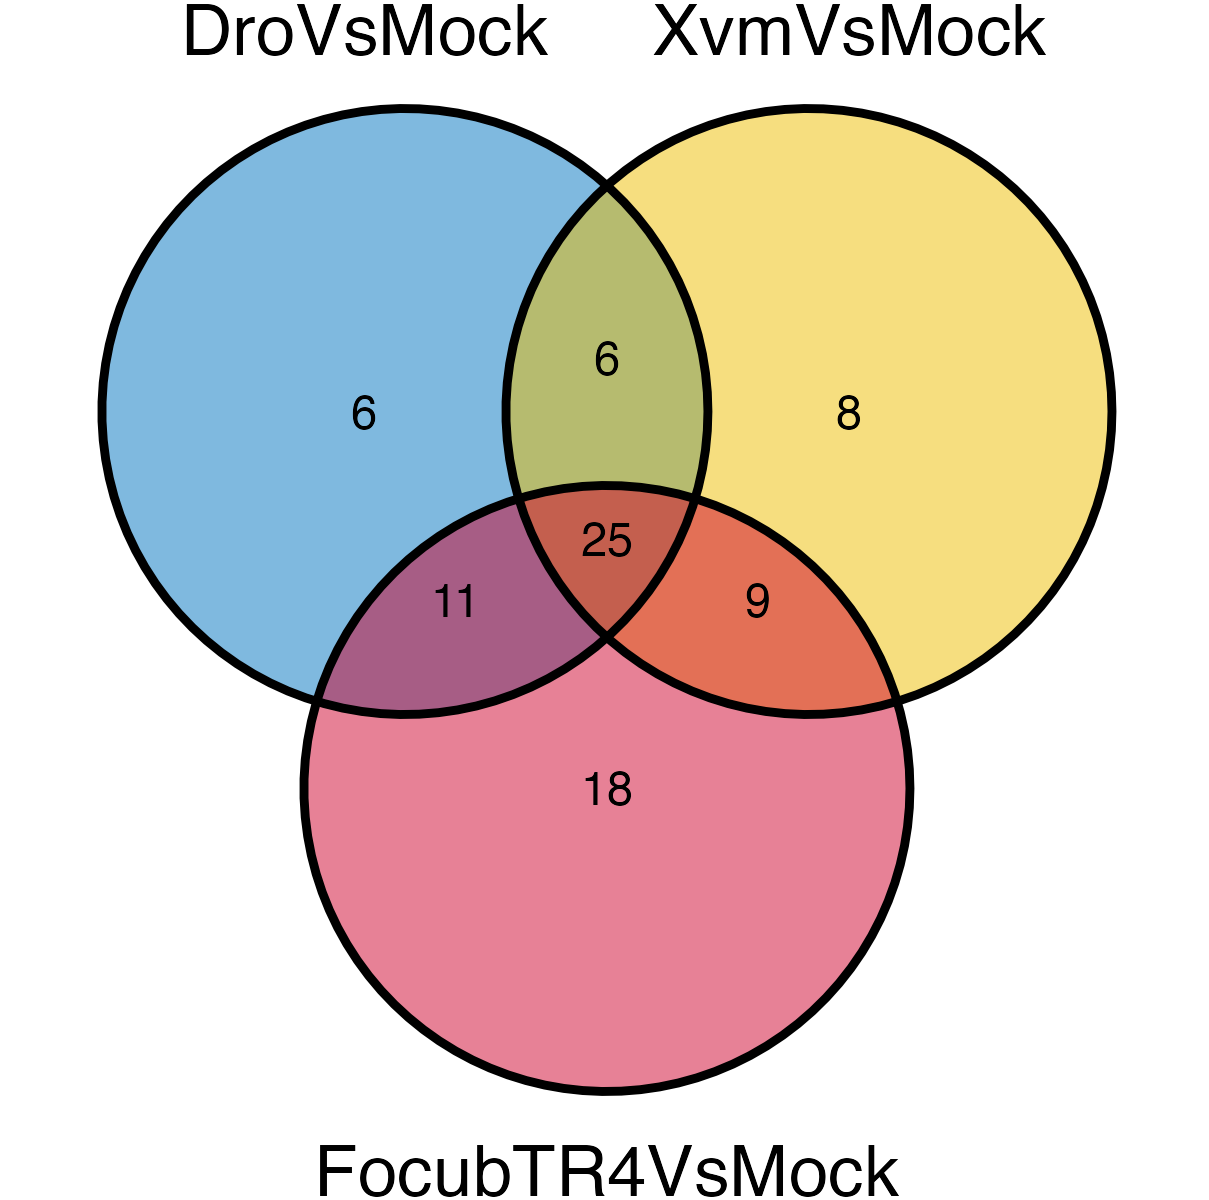
\includegraphics[width=\textwidth]{Figures/Pairwise_SharedFeaturesVenn_SecondTimePoint.png}
        \caption{}
        \label{fig:PairwiseVenn-SecondTimePoint}
    \end{subfigure}
    \caption[Distribution of significant features at the second time point (positive mode).]{\textbf{Distribution of significant features ($p \le0.05$) at the second time point (positive mode).}
    Utilising the 171 significant features ($p \le0.05$) identified through the one-way \ac{anova} conducted on features at the second time point, each treatment was compared to the mock-inoculated mock for pairwise analysis.
    \textbf{\subref{fig:DroVsCon_t-test}}) shows features of interest ($p \le0.05$) from drought-stress vs mock-inoculated pairwise analysis;
    \textbf{\subref{fig:XvmVsCon_t-test}}) shows features of interest ($p \le0.05$) from the \acl{xvm}-inoculated vs mock-inoculated pairwise analysis; 
    \textbf{\subref{fig:FocVsCon_t-test}}) shows features of interest ($p \le0.05$) from the \acl{Focub4}-inoculated vs mock-inoculated pairwise analysis. The red circles represent features above the $p \le0.05$ threshold. The $p$ values are transformed by $-log10$ so that the features of interest are plotted higher on the graph.
    \textbf{\subref{fig:PairwiseVenn-SecondTimePoint}}) Venn diagram depicting shared/potentially unique features of interest ($p \le0.05$) in drought-stressed (blue), \ac{xvm}-inoculated (yellow), or \ac{Focub4}-inoculated (red) plants compared to mock-inoculated plants at the second time point. 
    Panels \subref{fig:DroVsCon_t-test}, \subref{fig:XvmVsCon_t-test}, and \subref{fig:FocVsCon_t-test} were generated using MetaboAnalyst (v6.0).  
    }
    \label{fig:enter-label}
\end{figure}

\subsubsection{P1}

Of the 18 features of interest potentially unique to \ac{Focub4}-inoculated group, M449.365T1540.699 and M535.447T1540.43 emerged as potentially discriminant features. These features have the same retention time (25.67 minutes) and were not identified as features of interest in the \ac{xvm}-inoculated to mock-inoculated pairwise comparison, or the drought-stressed to mock-inoculated pairwise comparison. Further, M449.365T1540.699 was one of the six features shared between the first and second-time points. 

In our pairwise analysis, we assessed the \acf{fc} of all significant features at the second time point (n=171) in \ac{Focub4}-inoculated, \ac{xvm}-inoculated, or drought-stressed plants to the mock-inoculated plants, as \ac{fc} can be used to indicate a relationship between features with a similar retention time. M449.365T1540.699 did not meet the \ac{fc} threshold of $\ge2.0$, so was not captured as part of the \ac{fc} analysis. However,  M535.447T1540.43 was identified as part of the \ac{Focub4}-inoculated to mock-inoculated \ac{fc} analysis. This feature, M535.447T1540.43, exhibited an \ac{fc} of 2.3175 compared to the mock-inoculated plants. M535.447T1540.43 to M449.365T1540.699 shows a loss of 86Da (\ch{535->449}), which does not correspond to any common \ac{lcms} positive mode adducts, contaminants, or mass differences (e.g. hexose, 162Da; glucose, 180Da; water 18Da). The intensities of features eluting at 25.67 minutes were too low ($\geq800$, $\leq2000$) to identify fragmentation patterns of adducts from noise (threshold 400), also resulting in the absence of MS2 data. Nonetheless, M449.365T1540.699 and M535.447T1540.43 remain potentially discriminant features.

\subsubsection{P2}

Four additional features of interest potentially unique to \ac{Focub4}-inoculated plants, eluted at the same retention time (24.55 - 24.56 minutes), with $m/z$ values of 423.321, 605.416, 629.459, and 629.463. An additional feature of interest potentially unique to \ac{Focub4}-inoculated plants, M629.464T1456.367, was also included in the P3 set as it eluted at 24.2 minutes and shared the same mass ($m/z$: 629.464) as two features identified in the 24.55 to 24.56-minute window ($m/z$: 629.459, and 629.463). These features were also identified in the list of 19 metabolites potentially shared between the first and second time points, making them possible discriminatory candidates. However, two further features (M330.261T1473.013 and M575.479T1473.048) that had a retention time of 24.55 minutes were identified in drought-stressed to mock-inoculated pairwise comparison as well as \ac{Focub4}-inoculated to mock-inoculated pairwise comparison. Additionally, one feature (M628.514T1473.756) with a retention time of 24.55 minutes was identified in the \ac{xvm}-inoculated to mock-inoculated pairwise comparison, and \ac{Focub4}-inoculated to mock-inoculated pairwise comparison. The shared retention times suggest these features could be from the same metabolite.

Using an \ac{fc} threshold of $\ge2.0$, we compared the \ac{fc} of features of interest in drought-stressed, \ac{Focub4}-inoculated, or \ac{xvm}-inoculated plants, to mock-inoculated plants that eluted at 24.55 minutes. While the two features identified in both \ac{Focub4}-inoculated and drought-stressed plants (M330.261T1473.013 and M575.479T1473.048) did not exhibit an \ac{fc} of $\geq2.0$, the feature shared between \ac{Focub4}-inoculated and \ac{xvm}-inoculated plants (M628.514T1473.756) displayed an \ac{fc} of $\geq2.0$ (\ac{xvm}-inoculated = 2.0742, \ac{Focub4}-inoculated = 2.327), suggesting a these features are from the same metabolite. 
 
Unfortunately, due to low intensities ($\geq800$, $\leq2000$), MS2 data were unavailable for features eluting between 24.55 and 24.56 minutes. Moreover, identifying fragmentation patterns of adducts from noise (threshold 400) proved challenging. However, the features that eluted at 24.55 minutes are likely from the same metabolite and therefore will not distinguish \ac{Focub4}-inoculated plants from the other wilting stresses.

\subsubsection{P3}

Although the set of potentially unique features specific to \ac{xvm}-inoculated plants was limited (n=8), M682.262T843.183 emerged as a possible discriminant feature, with no other features of interest detected at similar retention times in other treatment groups. Moreover, M682.262T843.183 shared a retention time (14.05 minutes) with significant features identified across both the first and second time points. Despite this, M682.262T843.183 did not meet the fold change (\ac{fc}) threshold of $\geq2.0$, and similar to P1 and P2, exhibited low peak intensities falling within the range of $\geq800$ to $\leq2000$.

In negative mode data, five features with a similar retention time (14.05 minutes) were also identified as significant in \ac{xvm}-inoculated samples compared to the mock-inoculated samples, albeit exclusively at the second time point. Once more, these features displayed low peak intensities within the range of $\geq800$ to $\leq3000$.

\subsubsection{P4}

M386.164T943.456 was identified as a feature potentially unique to drought-stressed plants, eluting at 15.7 minutes. No features of interest with a similar retention time were found in the pairwise comparisons between \ac{xvm} and mock-inoculated samples, and \ac{Focub4} and mock-inoculated samples. The retention time of 15.7 minutes aligns with one of the 19 metabolites potentially shared between the first and second time points, suggesting M386.164T943.456 is a potential discriminatory candidate. Additionally, M386.164T943.456 exhibited an \ac{fc} of 3.9157 compared to the mock-inoculated samples. Consistent with previous findings, the peak intensities for M386.164T943.456 were low, falling within the range of $\geq800$ to $\leq2000$. 

%\subsection{Multispectral imaging as an approach for early symptom detection.}

%Multispectral imaging represents a promising approach for the early detection of symptoms in plant pathology. Despite our rigorous analysis, we were unable to discern any significant differences between the various treatments before the naked eye.  \textcolor{red}{I need to show the images here and talk about the lack of obvious difference.} This suggests that further refinement or complementary techniques may be necessary to enhance the sensitivity of multispectral imaging for early symptom detection in our experimental setup. 

%\subsubsection{Multispectral imaging does not distinguish symptoms between different wilting stresses.}

%One of the primary objectives of this study was to investigate whether multispectral imaging could differentiate between different types of wilting stresses. However, our findings indicate that multispectral imaging did not effectively distinguish between the symptoms induced by various wilting stresses. \textcolor{red}{Here I can talk about the time of symptom development, but need to remember for discussion that growers are unlikely to image over time and the environmental factors will affect the speed of disease progression too quickly to make this a viable option.}
%This underscores the complexity of symptom manifestation and suggests the need for alternative approaches or additional parameters to improve the discriminatory power of multispectral imaging in distinguishing between different types of wilting stresses.

\newpage
\section{Discussion and conclusion}

\Acf{um} was employed to study the metabolome of 'Grande Naine' banana plants subjected to three wilting stresses: \acl{fwb}, \textit{Xanthomomas} wilt of banana, and drought stress, at three different time points. Several potentially discriminant features shared between the first and second time points were identified. It is important to emphasise that these findings warrant further exploration, and we are not positing them as definitive biomarker candidates. Our investigation serves as an initial trial of \ac{um} to study the banana-wilt metabolome and putative biomarker candidates require validation. 

Before metabolite extraction, we measured internal and external symptom development in plants inoculated with \ac{Focub4} at 15, 18, and 21 \ac{dpi}, as well as on plants subjected to \ac{xvm}-inoculation, drought stress, and mock-inoculation at 7, 10, and 13 \ac{dpi}. \ac{Focub4} and \ac{xvm} are both causal agents of vascular wilts. \textcite{Biruma2007}, among others (see section \ref{section:BiomakerIntro}), have reported that distinguishing the symptoms of these wilts can be challenging for banana growers. Consistent with symptoms of \ac{Focub4} and \ac{xvm} infection described in the literature \parencite{Ploetz2015a, Garcia-Bastidas2019, Ordonez2015a, Ocimati2022, Tripathi2021}, our observations revealed different symptom profiles for each pathogen. \ac{xvm} infections were marked by rapid wilting, whereas \ac{Focub4} infections typically exhibited chlorotic patches and streaks, initiating from the lower leaf canopy. Furthermore, the progression of \ac{xvm} infections outpaced that of \ac{Focub4}, though this may be attributed to differences in inoculation protocols. Symptom development in drought-stressed plants surpassed the pace of both pathogen-induced wilts, likely attributable to the severity of the drought stress treatment.  

Symptom scores exhibited variability across different assessment types and treatments. While the method developed by \textcite{Garcia-Bastidas2019} was useful for comparing overall symptom development, it did not capture the nuanced differences in symptoms between \ac{xvm} and \ac{Focub4} infections. We note that \textcite{Garcia-Bastidas2019} did not suggest that their symptom scoring method can be used to compare different wilting stresses.

\bigskip
\noindent
Metabolites were extracted from lamina samples that were collected from four plants per treatment at each time point. Possible contaminants were identified in \ac{lcms} data from samples C12-2 and X12-4, so these samples were excluded from the analysis. Following aligned feature identification (see section \ref{sec:XCMS}), eight outliers were identified and removed (see Appendix C\ref{apx:outliers}). The removal of these outliers reduced the dataset, which inevitably decreased the robustness of our statistical analysis. Particularly in the pairwise comparisons of significant features identified at the second sampling time point (positive mode data), as the treatment groups were compared against only two mock-inoculated samples. It is for this reason we refer to features identified as part of the pairwise analysis with $p \le 0.05$ as "features of interest", rather than statistically significant features. Using this approach, we recorded 25 features of interest present in all pairwise comparisons (\ac{Focub4}-inoculated to mock-inoculated, \ac{xvm}-inoculated to mock-inoculated, drought-stressed to mock-inoculated), 18 that were potentially unique to \ac{Focub4}-inoculated plants, eight that were potentially unique to \ac{xvm}-inoculated plants, and six that were potentially unique to drought-stressed plants. 

Three sets of discriminatory features were identified using positive mode data (P1, P3, P4), from an initial set of 2,294 aligned features. We searched for features with similar retention times in the negative mode data and identified some potentially shared features. However, in both positive and negative ion modes, the features identified displayed low peak intensities ( $\geq800$ to $\leq3500$), which made the identification of common mass differences (e.g. hexose, 162Da; glucose, 180Da; water 18Da), adducts, and contaminants challenging. Subsequently, our ability to generate putative molecular formulae, classify potential compounds, and corroborate positive mode features with those detected in negative mode was limited. 

The low peak intensities occurred for all features of interest described (P1-P4), and have been observed in previous untargeted \ac{lcms} analysis of 'Grande Naine' banana plants inoculated with \ac{Focub4} or \ac{xvm} that we have conducted (data not shown). To generate samples for \ac{um} analysis, six 75mm by 25mm sections of lamina were extracted from three leaves of each plant. These 75mm by 25mm sections were snap-frozen, lyophilized, ground to a powder, and homogenised to generate a single sample for each plant. Given that \ac{Focub4} and \ac{xvm} are vascular pathogens that colonise xylem vessels in banana roots and pseudostems \parencite{Li2011, Pegg2019}, we suggest that the low peak intensities were due to a dilution of signal and that future \ac{um} studies of banana wilts should also sample vasculature tissue. 

\textcite{Takahashi2020} highlights that many plant responses to drought stress take place in the vasculature, particularly abscisic acid signalling. \textcite{Notaguchi2015} reviewed the dynamics of long-distance signalling via plant vascular tissues and highlighted that many defence-related proteins are often identified in xylem and phloem exudates. Recently, \textcite{Lin2022} showed that mitogen-activated protein kinase (MAPK) phosphatase 1 (MKP1) and its target kinases MPK3 and MPK6 form a signalling cascade that activates lignin biosynthesis in vascular tissues to promote vascular resistance in both \textit{Arabidopsis} and rice when challenged with pathogenic species of \textit{Xanthomonas} that target the vasculature. Importantly, \textcite{Lin2022} did not see the same promotion of vascular defence responses in plants challenged with pathogens that target the plant mesophyll. Indeed, the only family of fungal effectors currently recognised in \ac{Fo} are \acfp{sixg}, originally identified in tomato xylem sap \parencite{Houterman2007}. Combined, this suggests that plant vasculature is a key infection battleground for wilt pathogens. It is reasonable to conclude that the vascular tissue should be the next tissue type assessed in any similar \ac{um} studies investigating banana wilts, and signals may not be as diluted as was observed in lamina samples.  

\bigskip
\noindent
To the best of our knowledge, no previous \ac{um} studies have been employed to investigate the effects of different wilting stresses on banana plants. It is therefore challenging to gauge how many discriminate features are reasonable when assessing the effects of various wilting stresses on the banana metabolome. \textcite{Sambles2017} employed a similar \ac{um} approach to that of the current study to reveal differences between trees tolerant and susceptible to ash dieback disease (caused by the fungus \textit{Hymenoscyphus fraxineus}). The authors identified six separate putative metabolites from the positive mode data that could distinguish tolerant and susceptible ash (\textit{Fraxinus excelsior}). It is of note that the authors sample from different ash genotypes, whereas all samples from the current study were collected from 'Grande Naine' banana plants. 

Given the type of tissue sampled, the low number of samples for some treatment groups, and relatively few time points, it is likely that other discriminate metabolites were missed. There remains scope for refinement in the sampling methodology, particularly concerning sampling tissue type. Furthermore, it is important to determine whether these unique features we identified are specific to 'Grande Naine' banana plants or can be identified in other varieties, if similar trends are observed in response to other \ac{Focub} races, and if unique features can serve as viable biomarkers. This foundational research sets the stage for future investigations aimed at exploring the metabolomic responses of banana plants to various wilting stresses, helping to ensure the sustainability and security of banana cultivation worldwide. 

% --- Cut from the intro --- %

%In our study, we employed phenomic analyses, including multispectral and RGB imaging, and \acf{um} analysis, to elucidate banana responses to various wilting stresses and help develop \ac{fwb} disease diagnostic methods.

%Multispectral and RGB imaging studies in banana been established for disease detection and diagnosis. \textcite{Johansen2014} developed an automatic banana identification software to aid in Banana Bunch Top Virus inspection and \textcite{Liao2018} employed hyperspectral images and machine learning to diagnose Banana Streak Virus at earlier stages of infection. \textcite{Ochoa2016} designed a hyperspectral imaging system for disease scanning on banana plants focusing on Black Sigatoka. \acp{uav}, RGB imaging, and Artificial Neural Networks have also been employed in the monitoring of Yellow Sigatoka \parencite{Calou2020}.  

%Recently, \acf{rs} disease diagnosis efforts in banana have focused on the identification of \ac{Focub} infection \parencite{Ye2020a, Ye2020b, Selvaraj2019}.  Ye et al (2020a,b) demonstrated that \ac{uav}-based multispectral imagery can be used to diagnose \ac{fwb}. The authors observed statistically significant differences (p > 0.05) between healthy and diseased plants using six different \acp{vi}. Using logistic regression models to describe the relationship between the \acp{vi} in healthy or diseased plants, the authors reported that the red-edge chlorophyll index had the best performance for identifying \ac{fwb}.  

%It is clear that spectral reflectance can be used to diagnose \ac{fwb} in banana. What is not clear, however, is what is happening from a biological perspective to cause the differences in spectra observed, and whether the changes in spectra can be distinguished from other biotic and abiotic stresses. For instance, as \ac{Focub} is a vascular pathogen, it is important to ensure that \ac{Focub} infection can be differentiated from drought stress and other vasucular wilt pathogens like \acf{xvm}. 

